\documentclass[aps,prl,floatfix,preprint,nofootinbib]{revtex4}
\usepackage{amsmath}
\usepackage{graphicx}
\usepackage[colorinlistoftodos]{todonotes}
\usepackage{indentfirst}
\usepackage{listings}
\usepackage{color}
\usepackage[title,titletoc,toc]{appendix}
\usepackage[hidelinks,hyperfootnotes=false,bookmarks=false]{hyperref}
\usepackage{epsfig}
\usepackage{setspace}

\setlength{\paperheight}{11in}

\definecolor{mykeyword}{rgb}{139, 0, 139}
\definecolor{mygray}{rgb}{0.5,0.5,0.5}
\lstset{ %
  backgroundcolor=\color{white},   % choose the background color; you must add \usepackage{color} or \usepackage{xcolor}
  basicstyle=\footnotesize,        % the size of the fonts that are used for the code
  breakatwhitespace=false,         % sets if automatic breaks should only happen at whitespace
  breaklines=true,                 % sets automatic line breaking
  captionpos=b,                    % sets the caption-position to bottom
  commentstyle=\color{blue},       % comment style
  deletekeywords={...},            % if you want to delete keywords from the given language
  escapeinside={\%*}{*)},          % if you want to add LaTeX within your code
  extendedchars=true,              % lets you use non-ASCII characters; for 8-bits encodings only, does not work with UTF-8
  frame=none,                      % adds a frame around the code
  keepspaces=true,                 % keeps spaces in text, useful for keeping indentation of code (possibly needs columns=flexible)
  keywordstyle=\color{mykeyword},  % keyword style
  language=c++,                    % the language of the code
  morekeywords={*,...},            % if you want to add more keywords to the set
  numbers=left,                    % where to put the line-numbers; possible values are (none, left, right)
  numbersep=5pt,                   % how far the line-numbers are from the code
  numberstyle=\tiny\color{mygray}, % the style that is used for the line-numbers
  rulecolor=\color{black},         % if not set, the frame-color may be changed on line-breaks within not-black text (e.g. comments (green here))
  showspaces=false,                % show spaces everywhere adding particular underscores; it overrides 'showstringspaces'
  showstringspaces=false,          % underline spaces within strings only
  showtabs=false,                  % show tabs within strings adding particular underscores
  stepnumber=1,                    % the step between two line-numbers. If it's 1, each line will be numbered
  stringstyle=\color{red},         % string literal style
  tabsize=2,                       % sets default tabsize to 2 spaces
  title=\lstname                   % show the filename of files included with \lstinputlisting; also try caption instead of title
}

\begin{document}
\title{Modeling Two Body Collisions with Spring Potential Interactions}
\author{Matthew \textsc{Epland}}
\email{mbe9@phy.duke.edu}
\author{ Douglas \textsc{Davis}}
\email{drd25@phy.duke.edu}
%\href{mailto:my_address@wikibooks.org}{my\_address@wikibooks.org}
\affiliation{Department of Physics, Duke University}
\date{\today}

\hypersetup{pdftitle=Modeling Two Body Collisions}
\hypersetup{pdfauthor={Matthew Epland, Douglas Davis}}
%\hypersetup{bookmarks=false}
\hypersetup{pdfkeywords={Classical Physics, Two Body Collisions}}

\begin{abstract}
  This paper describes a computational study of two body collisions where the dynamics of the bodies are governed by a Hooke's Law type force at the interaction points. We investigate a number of scenarios which involve both a stationary target mass which is stuck by a projectile mass with some horizontal velocity in a two dimensional plane, as well as scenarios where both masses are moving in towards each other. The masses trajectories are determined from a simulation software package, written by the authors, that models the force between the masses as they interact with each other based on the initial kinematic state of the system. Specific attention was given to the systems behavior with different initial projectile velocities, impact parameters, energy loss rates and power dependence in the force law.
\end{abstract}\maketitle
\section{Introduction}
When two classical objects physically collide they experience a normal force between them. In the simplest case, that of two spherical masses, the normal force is orthogonal to the surface and is in line with the center of mass for both the objects. The magnitude of the normal force between masses $m_{1}$, $m_{2}$ with radii $r_{1}$, $r_{2}$ can be modeled as $ \left| F \right| = k \left(\Delta x\right)^{\lambda}$, where $\Delta x = r_1 + r_2 - \left| \mathbf{x}^{(1)}-\mathbf{x}^{(2)} \right|$ is the displacement from equilibrium and $k$ is an effective spring constant. Setting $\lambda = 1$ results in the familiar Hook's Law spring force, but by including the $\lambda$ power dependence we are able to study a wider array of collisions, particularly those where the masses deform enough that the normal force between them becomes nonlinear. As the masses deform and push against each other some of the mechanical energy of the system may be lost to internal degrees of freedom, such as heat. One way to model these inelastic collisions is by including viscous damping proportional to the velocity, which was the method used in this study.

Any two body collision can be reduced to 2-dimensional motion in a plane containing both masses and their initial velocity vectors. Additionally, in this paper we limit ourselves to the case where the initial velocities are parallel, though the masses may be initially off center from each other by a distance $s$, the impact parameter. One of the masses, the target $m_{1}$, may be at rest initially, though we also allow it to have an initial closing velocity in some studies. For continence we pick our coordinate system such that all the initial velocities lie along $\hat{x}$ and the target is on the $\hat{y}$ axis, $y_{1}(t=0)=0$ (Figure~\ref{fig:schematic}).

\begin{figure}[htbc]
  \centering
  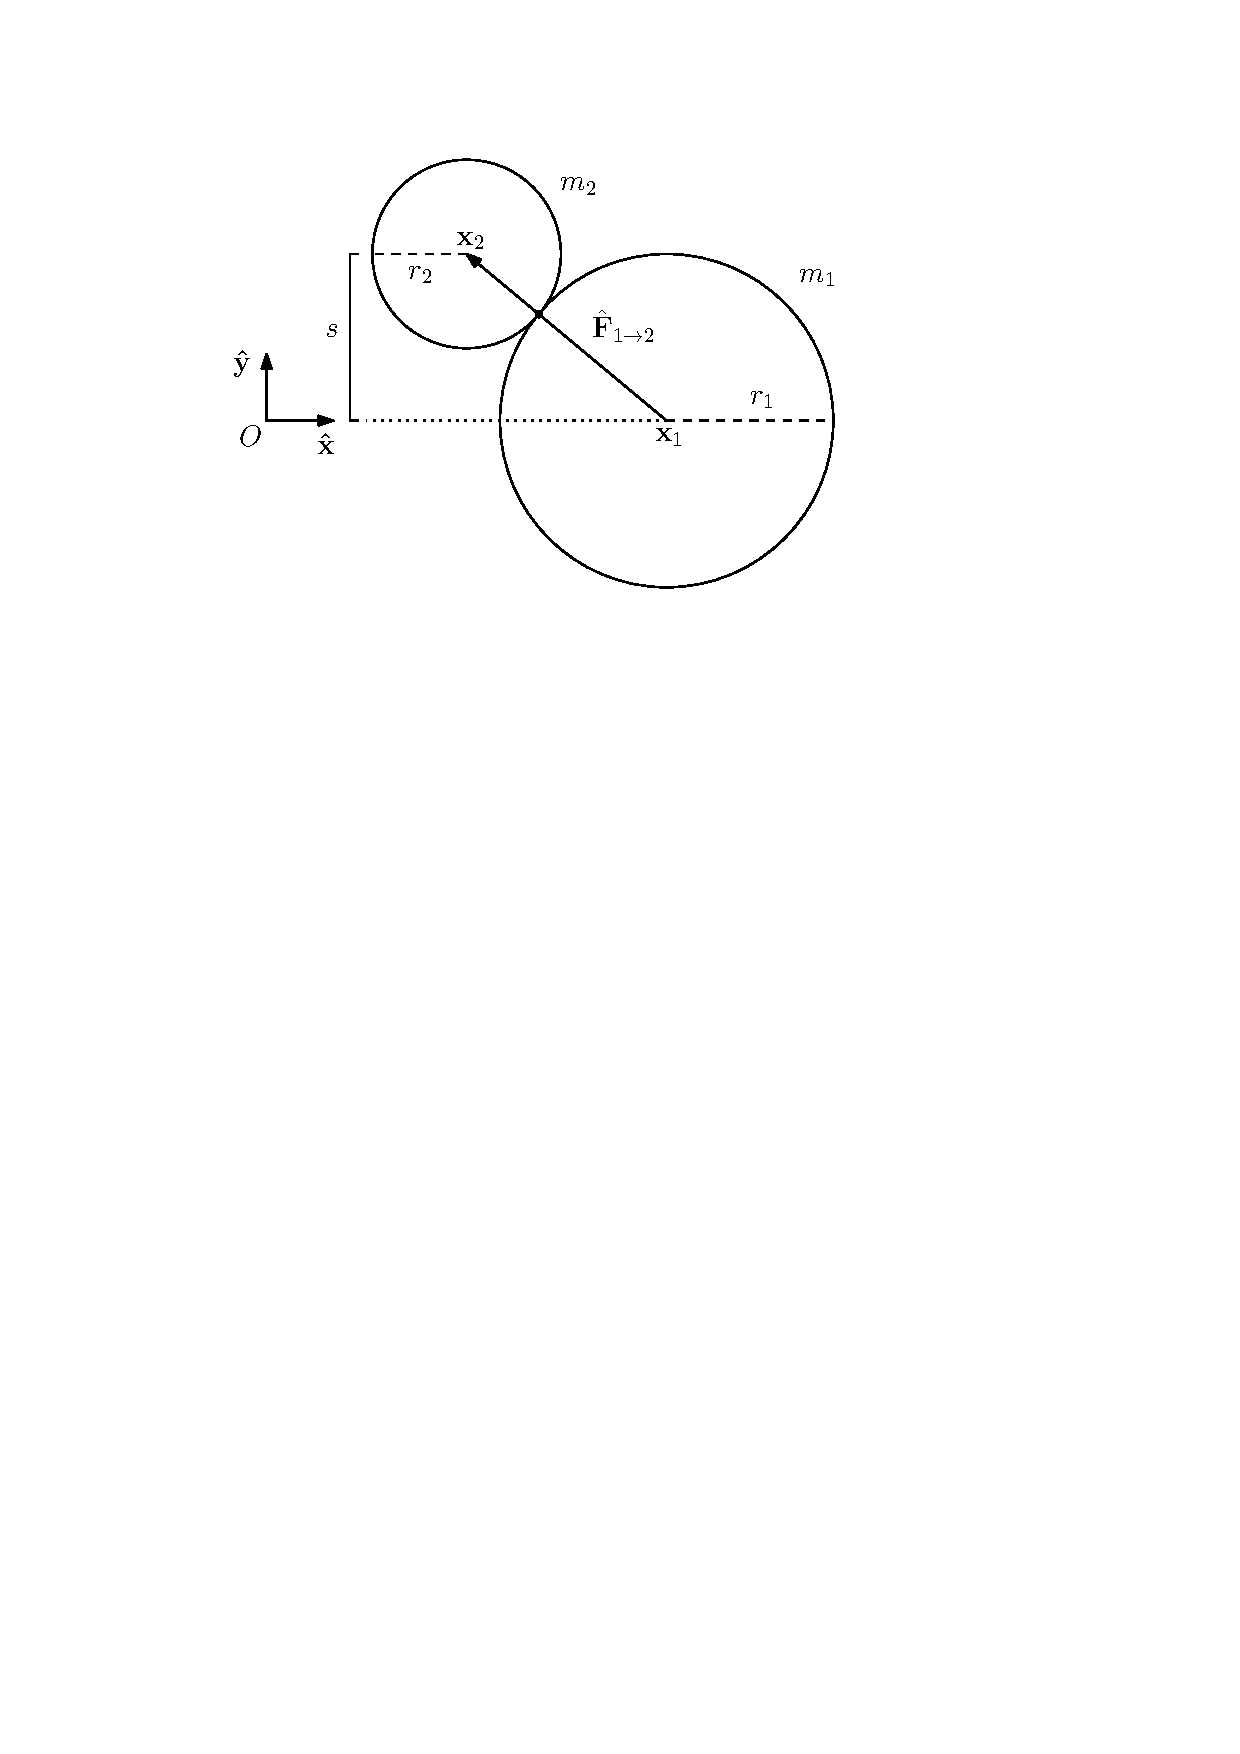
\includegraphics[width=.75\textwidth]{plots/cj_diag.pdf}
	          {\par\nobreak\rule[9pt]{35em}{0.5pt}\vspace{-5mm}}
	          \caption{Schematic View of the initial state at first contact, $t = 0$.}
	          \label{fig:schematic}
\end{figure}

In order to rapidly investigate the many possible variations of this seemingly simple two body collision a software simulation was chosen over attempting to solve each variation analytically. Written in \texttt{C++} and using some of the \texttt{ROOT}~\cite{ref_root} particle physics analysis libraries the simulation code at its core operates by iteratively calculating the object's change in position and velocity during a small time step, $\Delta t$, during which the acceleration is assumed to be constant. This is done by calculating $\Delta x$ \eqref{eq:displacement} from the $n-1$ positions, and then $\left|F\right|$ and the unit vector between the two masses centers $\mathbf{\hat{F}}_{j\rightarrow i}$ \eqref{eq:force}. Once the force has been estimated it is a simple matter to compute the $n$ time step positions \eqref{eq:position}, and velocities \eqref{eq:velocity}. When calculating the velocity we include a $\left(1-\eta\right)$ term to implement the viscous dampening energy losses were $\eta$ is the proportional decrease in velocity per time step.

\begin{equation}\label{eq:position}
  \mathbf{x}^{(i)}_{n} = \mathbf{x}^{(i)}_{n-1} + \dot{\mathbf{x}}^{(i)}_{n-1} \Delta t + \frac{1}{2m_i} \left| F \right| \mathbf{\hat{F}}_{j\rightarrow i} \left(\Delta t\right)^2
\end{equation}
\begin{equation}\label{eq:velocity}
  \dot{\mathbf{x}}^{(i)}_{n} = (1-\eta)\dot{\mathbf{x}}^{(i)}_{n-1} + \frac{1}{m_i} \left| F \right| \mathbf{\hat{F}}_{j\rightarrow i} \Delta t
\end{equation}
\begin{equation}\label{eq:displacement}
  \Delta x_{n-1} = r_1 + r_2 - \left| \mathbf{x}^{(1)}_{n-1}-\mathbf{x}^{(2)}_{n-1} \right|
\end{equation}
\begin{equation}\label{eq:force}
  \left| F \right| = k \left(\Delta x_{n-1}\right)^{\lambda},\quad \mathbf{\hat{F}}_{j\rightarrow i} = \frac{\mathbf{x}^{(i)}_{n-1}-\mathbf{x}^{(j)}_{n-1}}{\left|\mathbf{x}^{(i)}_{n-1}-\mathbf{x}^{(j)}_{n-1}\right|}
\end{equation}

In addition to the position and velocity of the masses we also calculate their kinetic energies and the potential energy stored in the deformed bodies, e.g. spring \eqref{eq:energy}. The force is conservative, so $\mathbf{F} = - \nabla V \rightarrow V = \int \left|F\right| d\left(\Delta x\right)$. With a small enough $\Delta t$ these iterative equations model the physics of the interaction very well. To ensure that $\Delta t$ is not set too large the code checks each masses change in position at every time step. If the change in position is larger than 1\% of the masses radius a warning is generated and the simulation is re-run with a smaller $\Delta t$. Throughout the rest of this paper SI units are assumed where none are given.
\begin{equation}\label{eq:energy}
  V_n = \frac{k}{\lambda+1}\left(\Delta x_n\right)^{\lambda+1},\quad T_n = \frac{m_1}{2}\left(\dot{\mathbf{x}}^{(1)}_n\right)^2 + \frac{m_2}{2}\left(\dot{\mathbf{x}}^{(2)}_n\right)^2
\end{equation}

\section{Results}
\subsection{Simulation Performance}
\subsubsection{Default Configuration}
One of the first tasks was to validate the simulation framework using a system where the physics was simple and easy to intuitively predict. This system uses a stationary target of radius 2, with a projectile of radius 1 incoming at velocity 5 with an impact parameter of 1. The objects have equal density. We configure this system to have no energy loss ($\eta = 0$), $\lambda=1$ power law, and $k=100$ force constant. $\Delta t = 0.001$ was found to give sufficent precision for most studies and is the default $\Delta t$ value for all simulations unless otherwise noted. To begin to get an understanding of the collision we first plot each objects center of mass trajectory during the time when they are in contact with each other and are undergoing accelerations (Figure~\ref{fig:tracks_default}). The projectile rebounds off the target sending it off at a slow velocity in the oposite direction while the systems center of mass moves steadly in a straight line.
\begin{figure}[h!]
  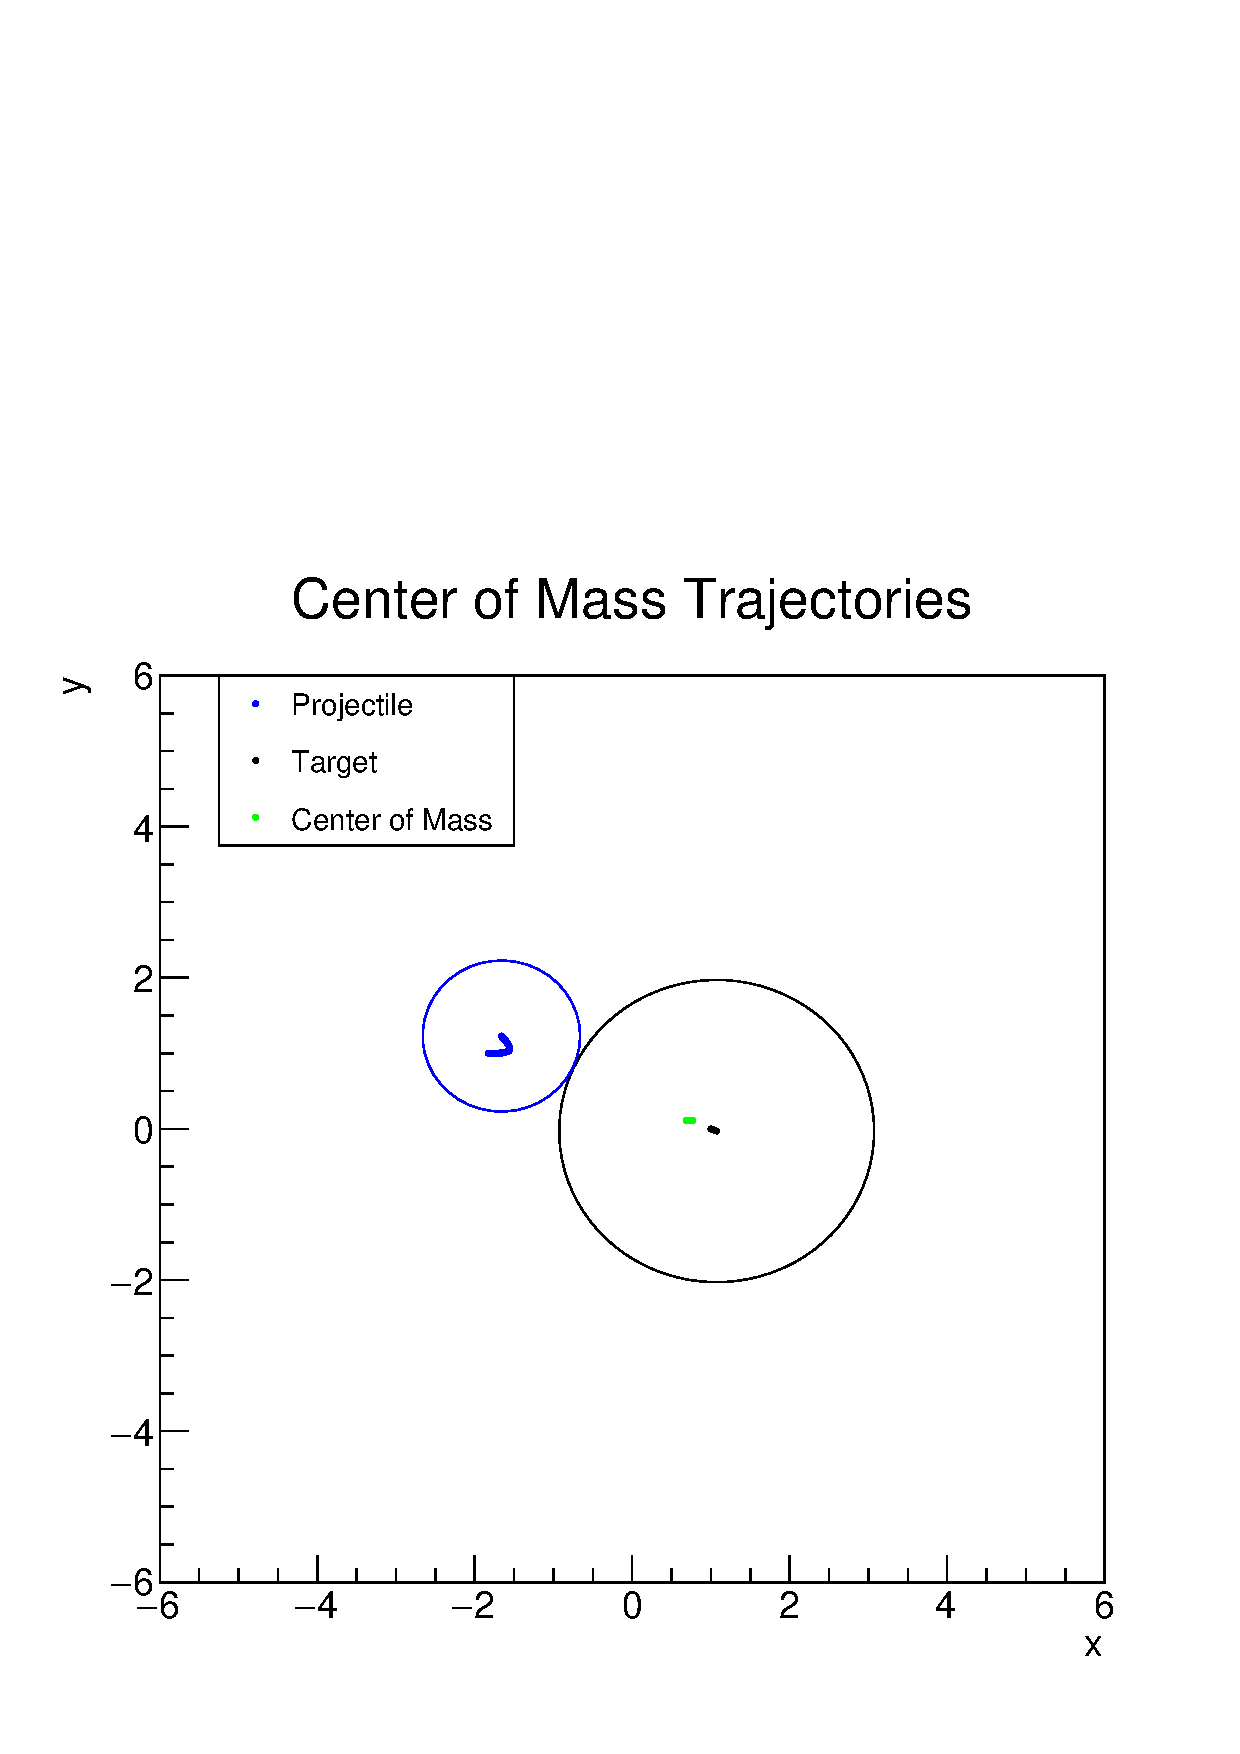
\includegraphics[width=.45\textwidth]{plots/default/x_vs_y_with_ellipse.pdf}
  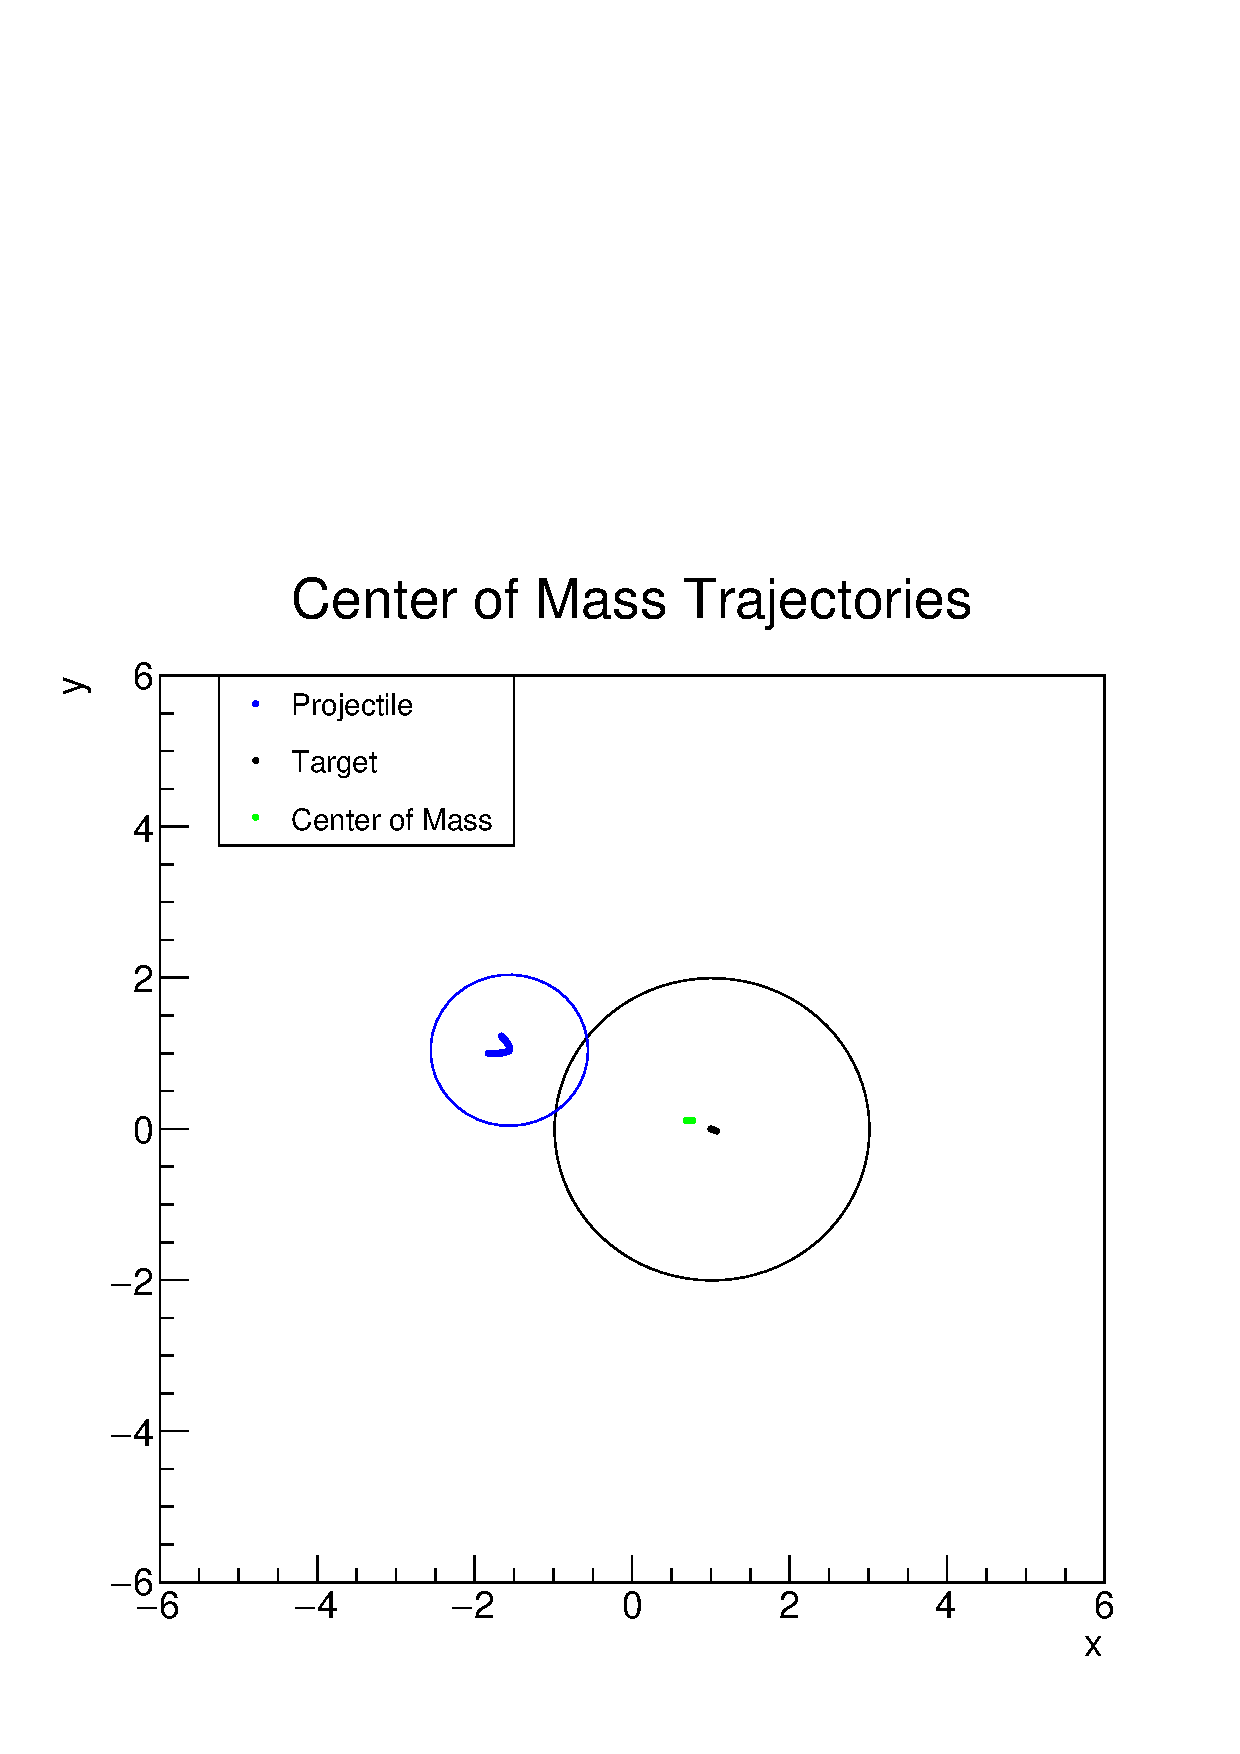
\includegraphics[width=.45\textwidth]{plots/default/x_vs_y_with_ellipse_MS.pdf}
                  {\par\nobreak\rule[9pt]{35em}{0.5pt}\vspace{-5mm}}
                  \caption{(L) The initial state of the system when the objects come in contact. The collections of points (which form a continuous line) show the position of the center of each object at each time step while the objects are in contact. (R) The state of the system when the objects are at a minimum separation i.e. maximum $\Delta x$ from equilibrium.}
                  \label{fig:tracks_default}
\end{figure}

Potential and kinetic energy of the system is tracked throughout the simulation steps giving us the ability to moniter total energy conservation. It also allows us to visualize the flow of energy throughout the system. For the default configuration, that energy flow is shown in Figure~\ref{fig:energy_default}. It can be seen that the total energy trend is not completely constant. This is believed to be from the approximate quality of the simulation using finite time steps. The discrepancy is very small.
\begin{figure}
  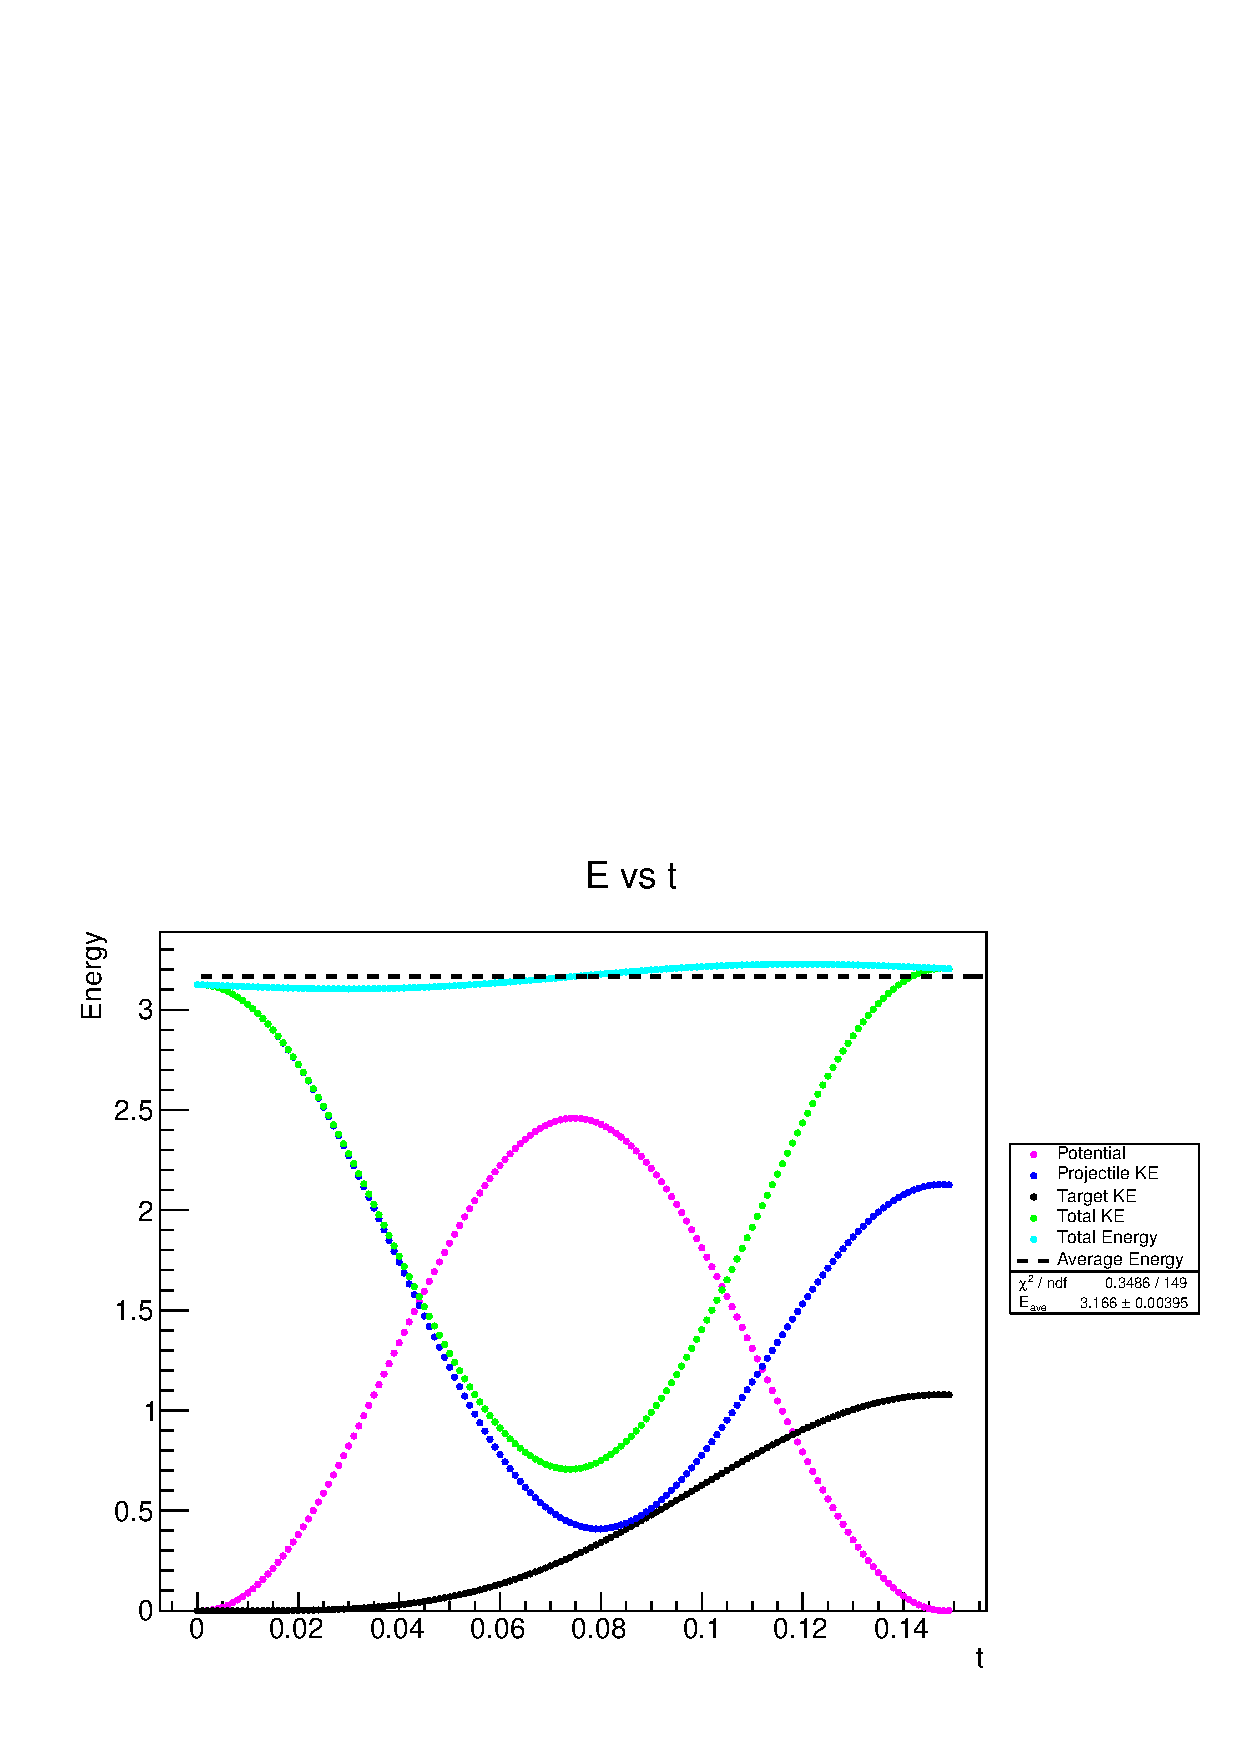
\includegraphics[width=.8\textwidth]{plots/default/E_vs_t.pdf}
                  {\par\nobreak\rule[9pt]{35em}{0.5pt}\vspace{-5mm}}
                  \caption{Trends for different energies in the system: object and total kinetic energies, potential energy, and the total energy of the system.}
                  \label{fig:energy_default}
\end{figure}

\subsubsection{Equal masses, zero net momentum}
Another system we investigated for validation was a system with two identical objects colliding with each other at equal but opposite velocities. In this system the objects have equal density with a radius of 1 and the initial velocities are $5$ and $-5$, respectively; the force constant was $k = 1000$ and $\lambda = 1$. The observed behavior is present in Figures~\ref{fig:tracks_c6}~and~\ref{fig:vx_c6}. The trends for the motions of the objects are as expected, specifically we were looking for antisymmetric velocity trends and constant system center of mass momentum.
\begin{figure}[h!]
  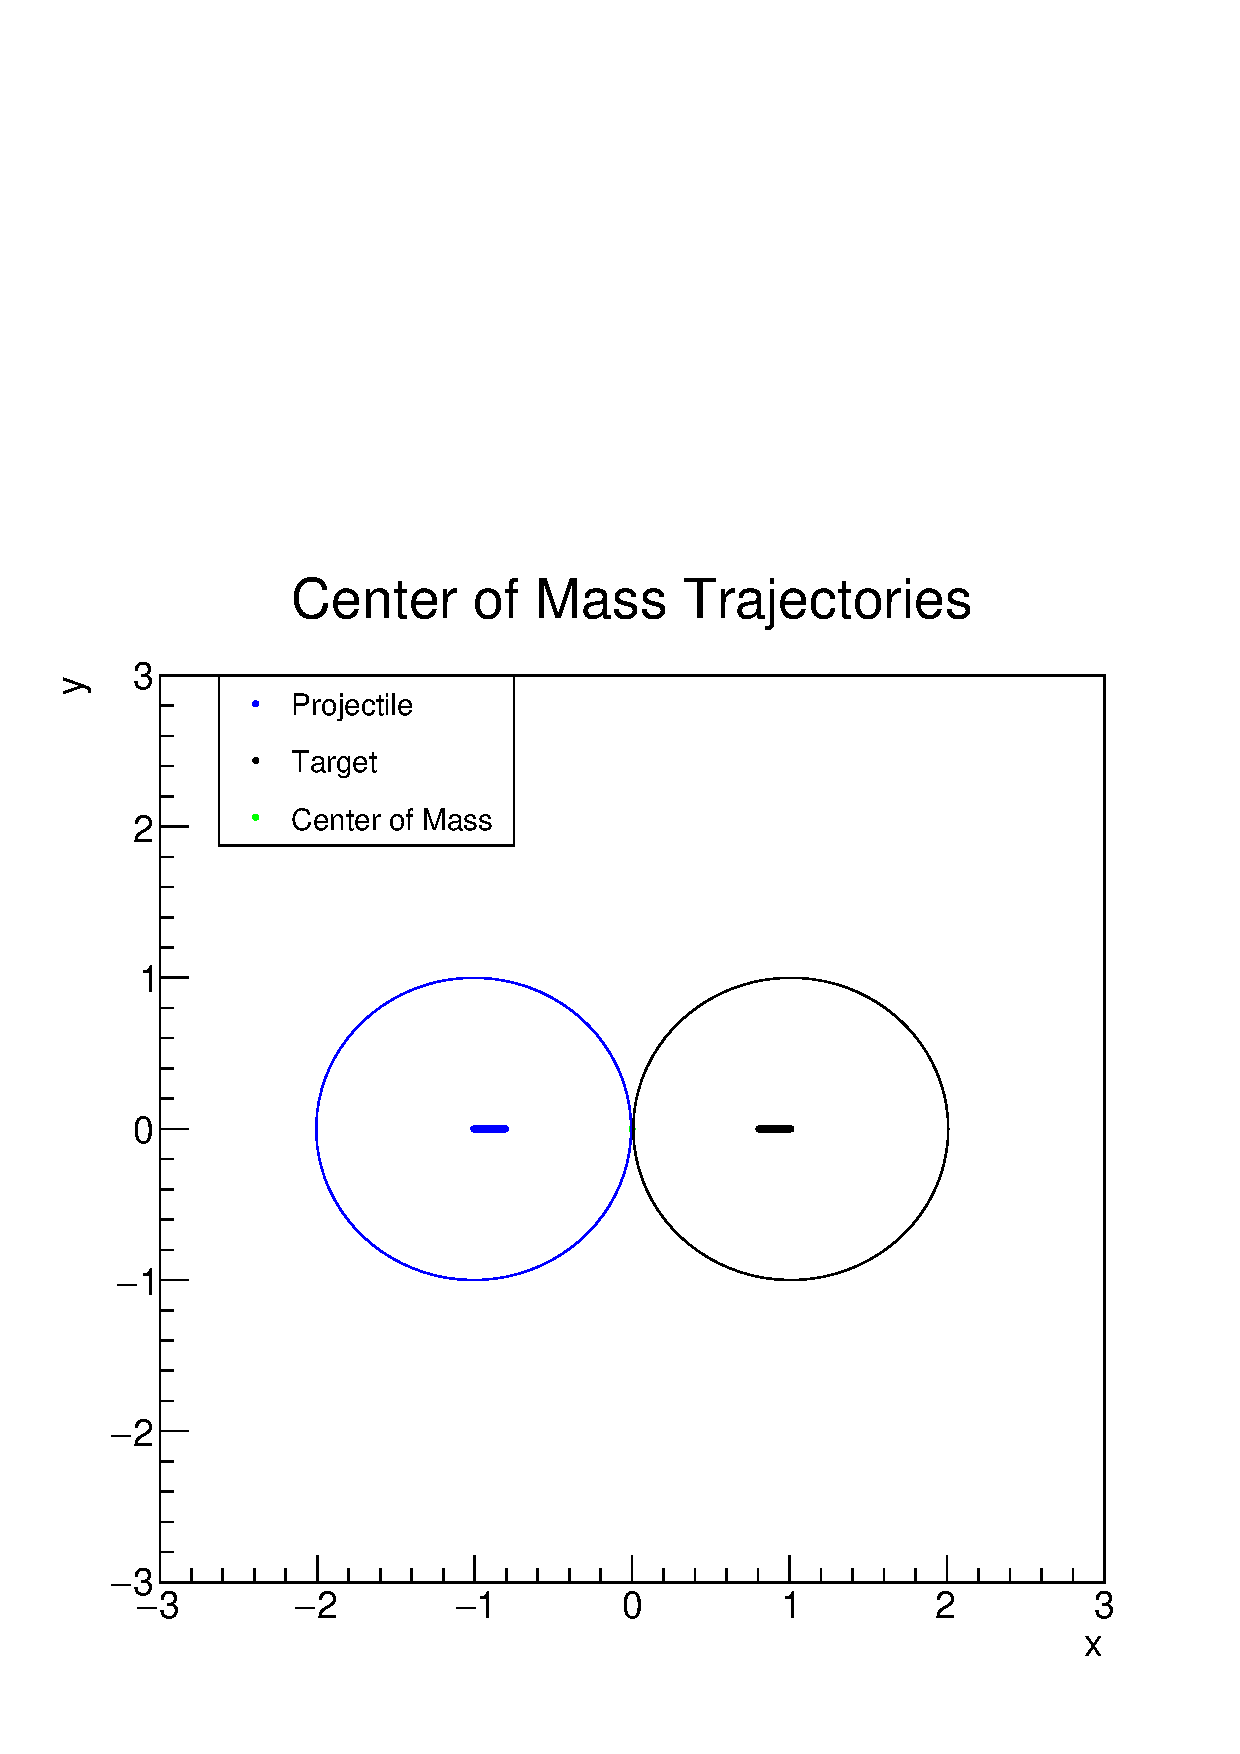
\includegraphics[width=.45\textwidth]{plots/out_c6/x_vs_y_with_ellipse.pdf}
  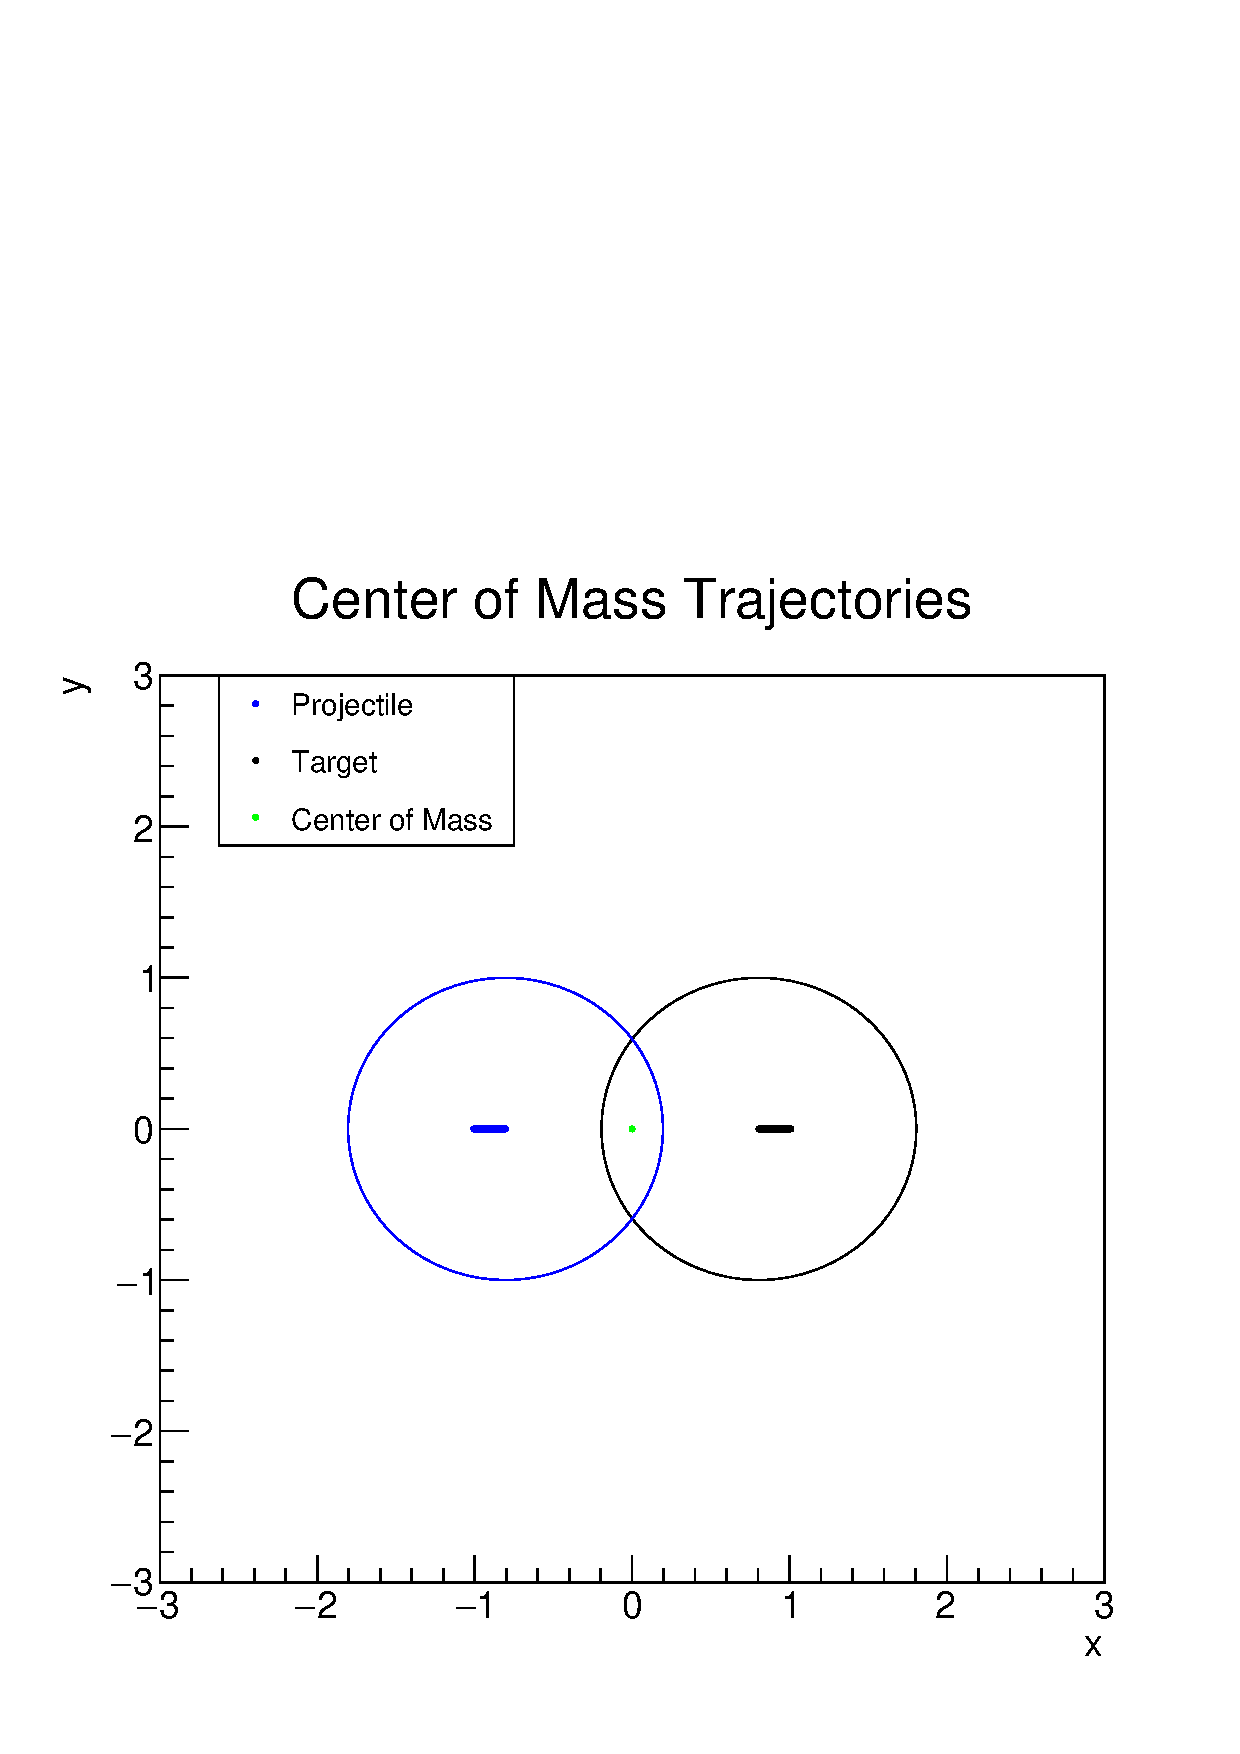
\includegraphics[width=.45\textwidth]{plots/out_c6/x_vs_y_with_ellipse_MS.pdf}
                  {\par\nobreak\rule[9pt]{35em}{0.5pt}\vspace{-5mm}}
                  \caption{(L) Object initial state, with tracks points (R) Objects at minimum separation, with track points}
                  \label{fig:tracks_c6}
\end{figure}
\begin{figure}[h!]
  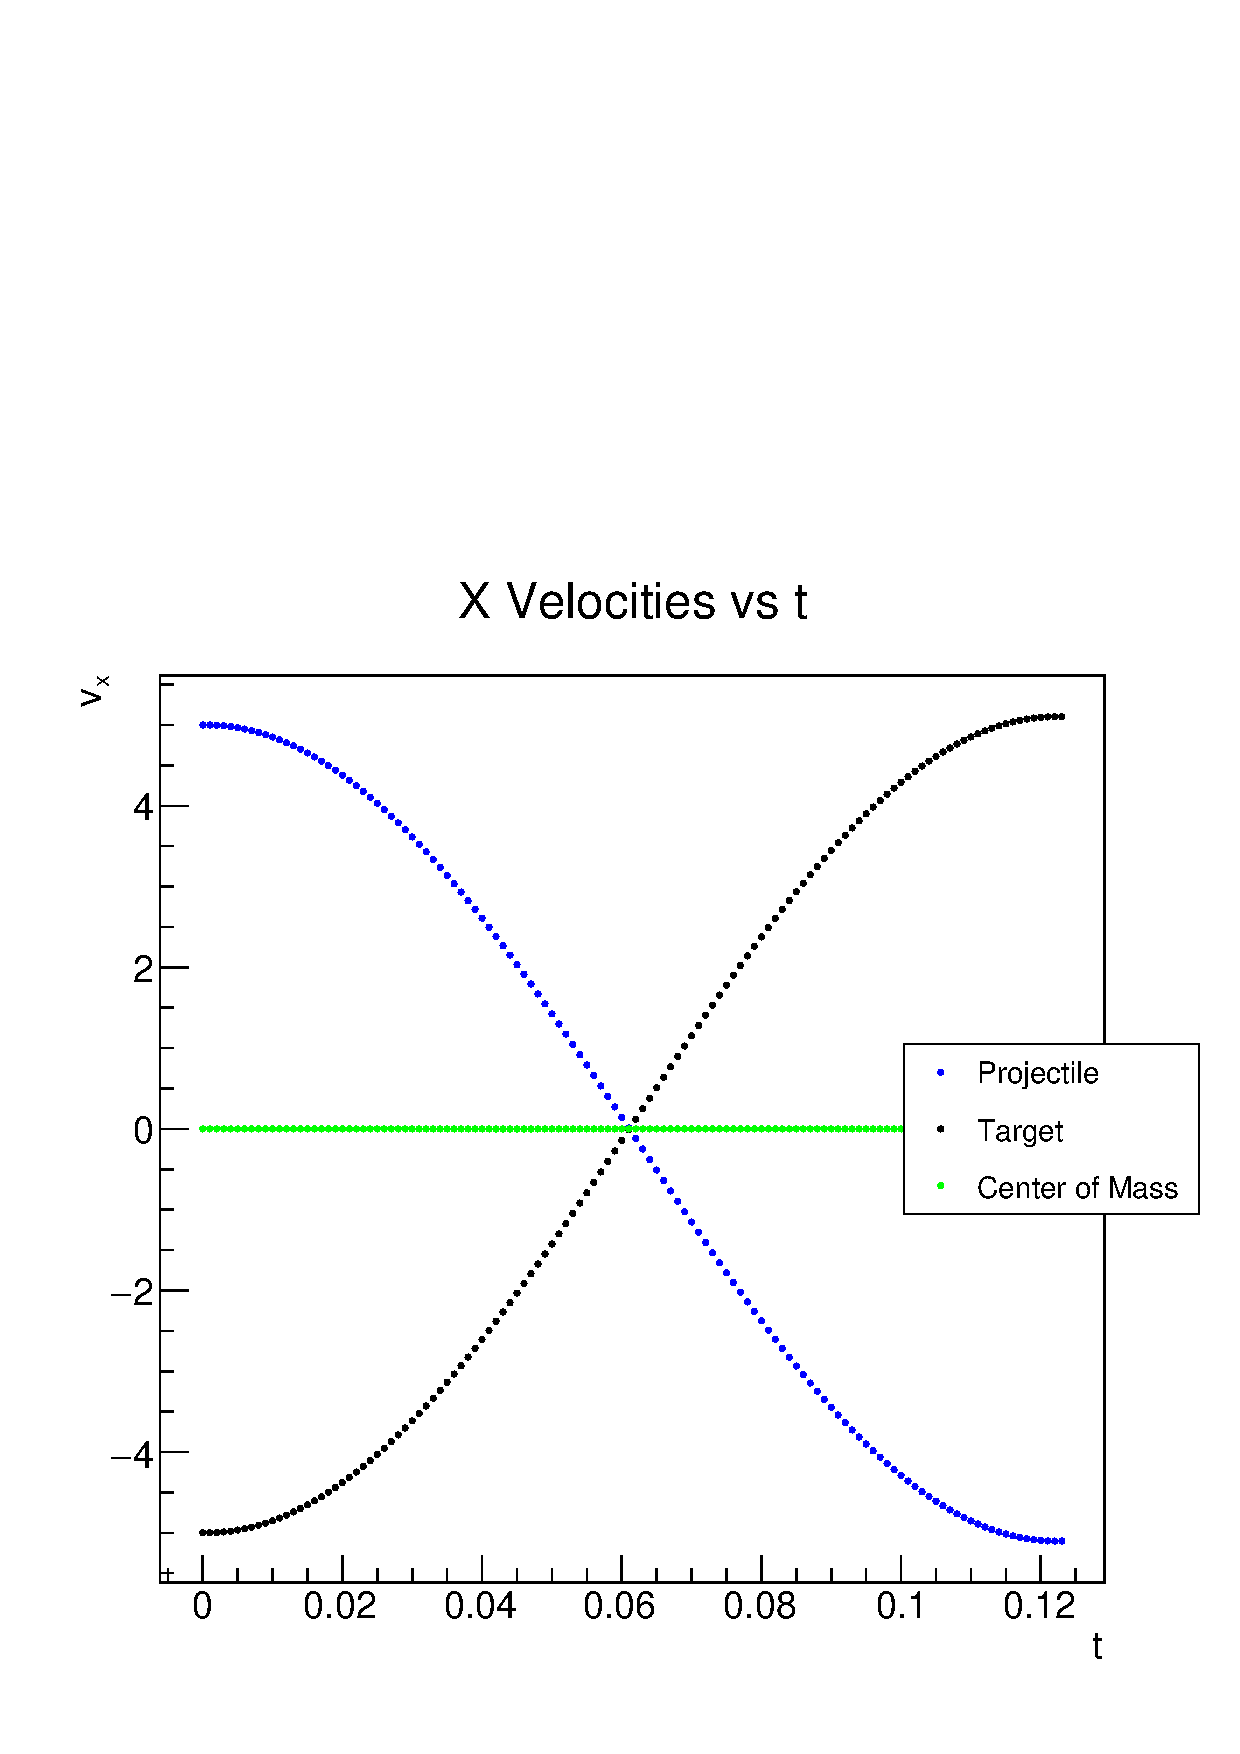
\includegraphics[width=.45\textwidth]{plots/out_c6/vx_vs_t.pdf}
                  {\par\nobreak\rule[9pt]{35em}{0.5pt}\vspace{-5mm}}
                  \caption{The velocity in the $x$ direction for both objects. The trend shows that the objects slow as the come together, come to rest, and move off in opposite directions again. As expected the system's center of mass velocity is zero.}
                  \label{fig:vx_c6}
\end{figure}

\subsubsection{Large, slow moving target with small, fast projectile}
The final validation system we investigated was made up of a target with mass 30 and radius 3 moving with velocity $-2$ and a projectile with mass 1 and radius 1 moving with velocity 8; the force constant was $k = 1000$ and $\lambda = 1$. The impact parameter was set to 0. For this system we were looking for large momentum transfer to the projectile (essentially being quickly turned around by the slightly effected target). Figure~\ref{fig:tracks_c7} shows the object trajectories. Figure~\ref{fig:vx_c7} shows the horizontal velocities for the system. As expectd, the large and slow target is slightly effected and its motion remains in the same direction, while the small and fast projectile is deflected against the target and moves away at a faster velocity compared to its incoming velocity.
\begin{figure}[h!]
  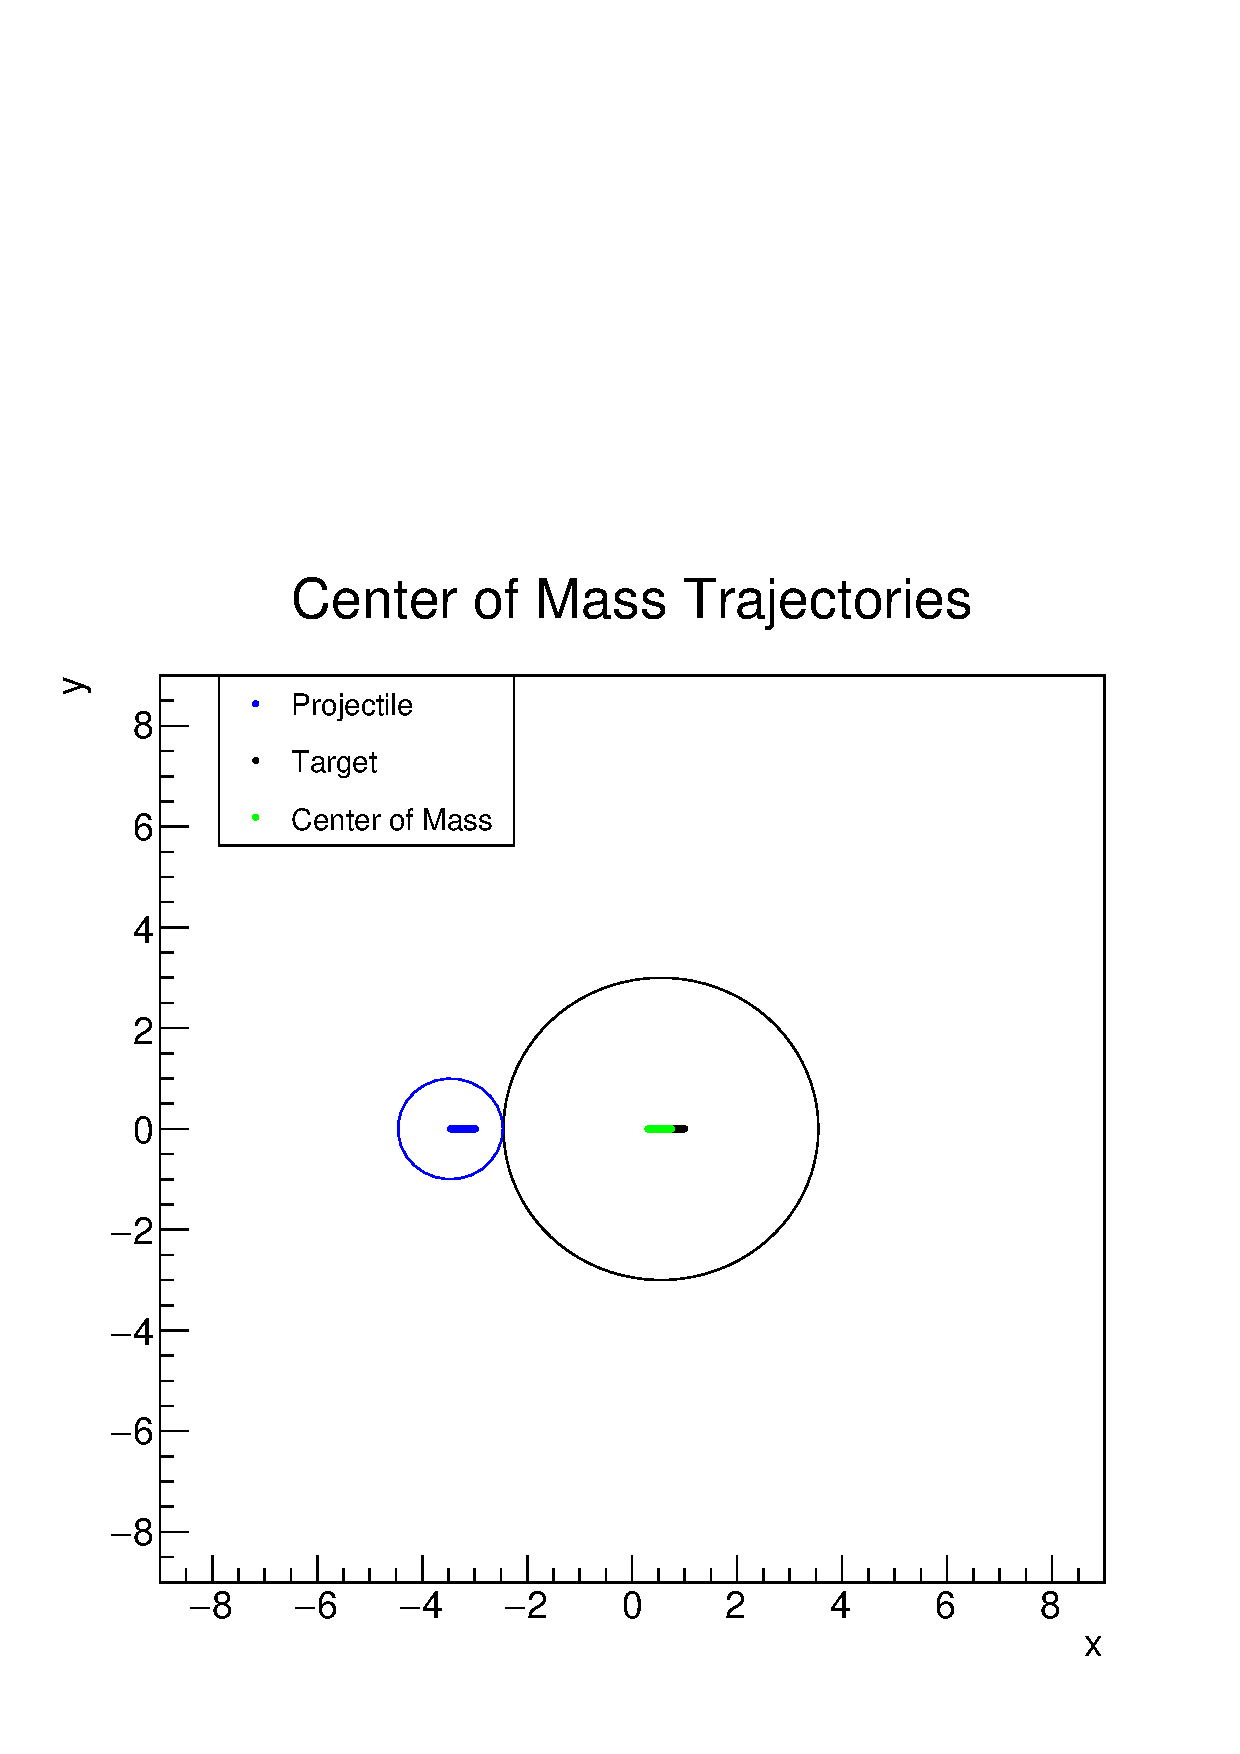
\includegraphics[width=.45\textwidth]{plots/out_c7/x_vs_y_with_ellipse.pdf}
  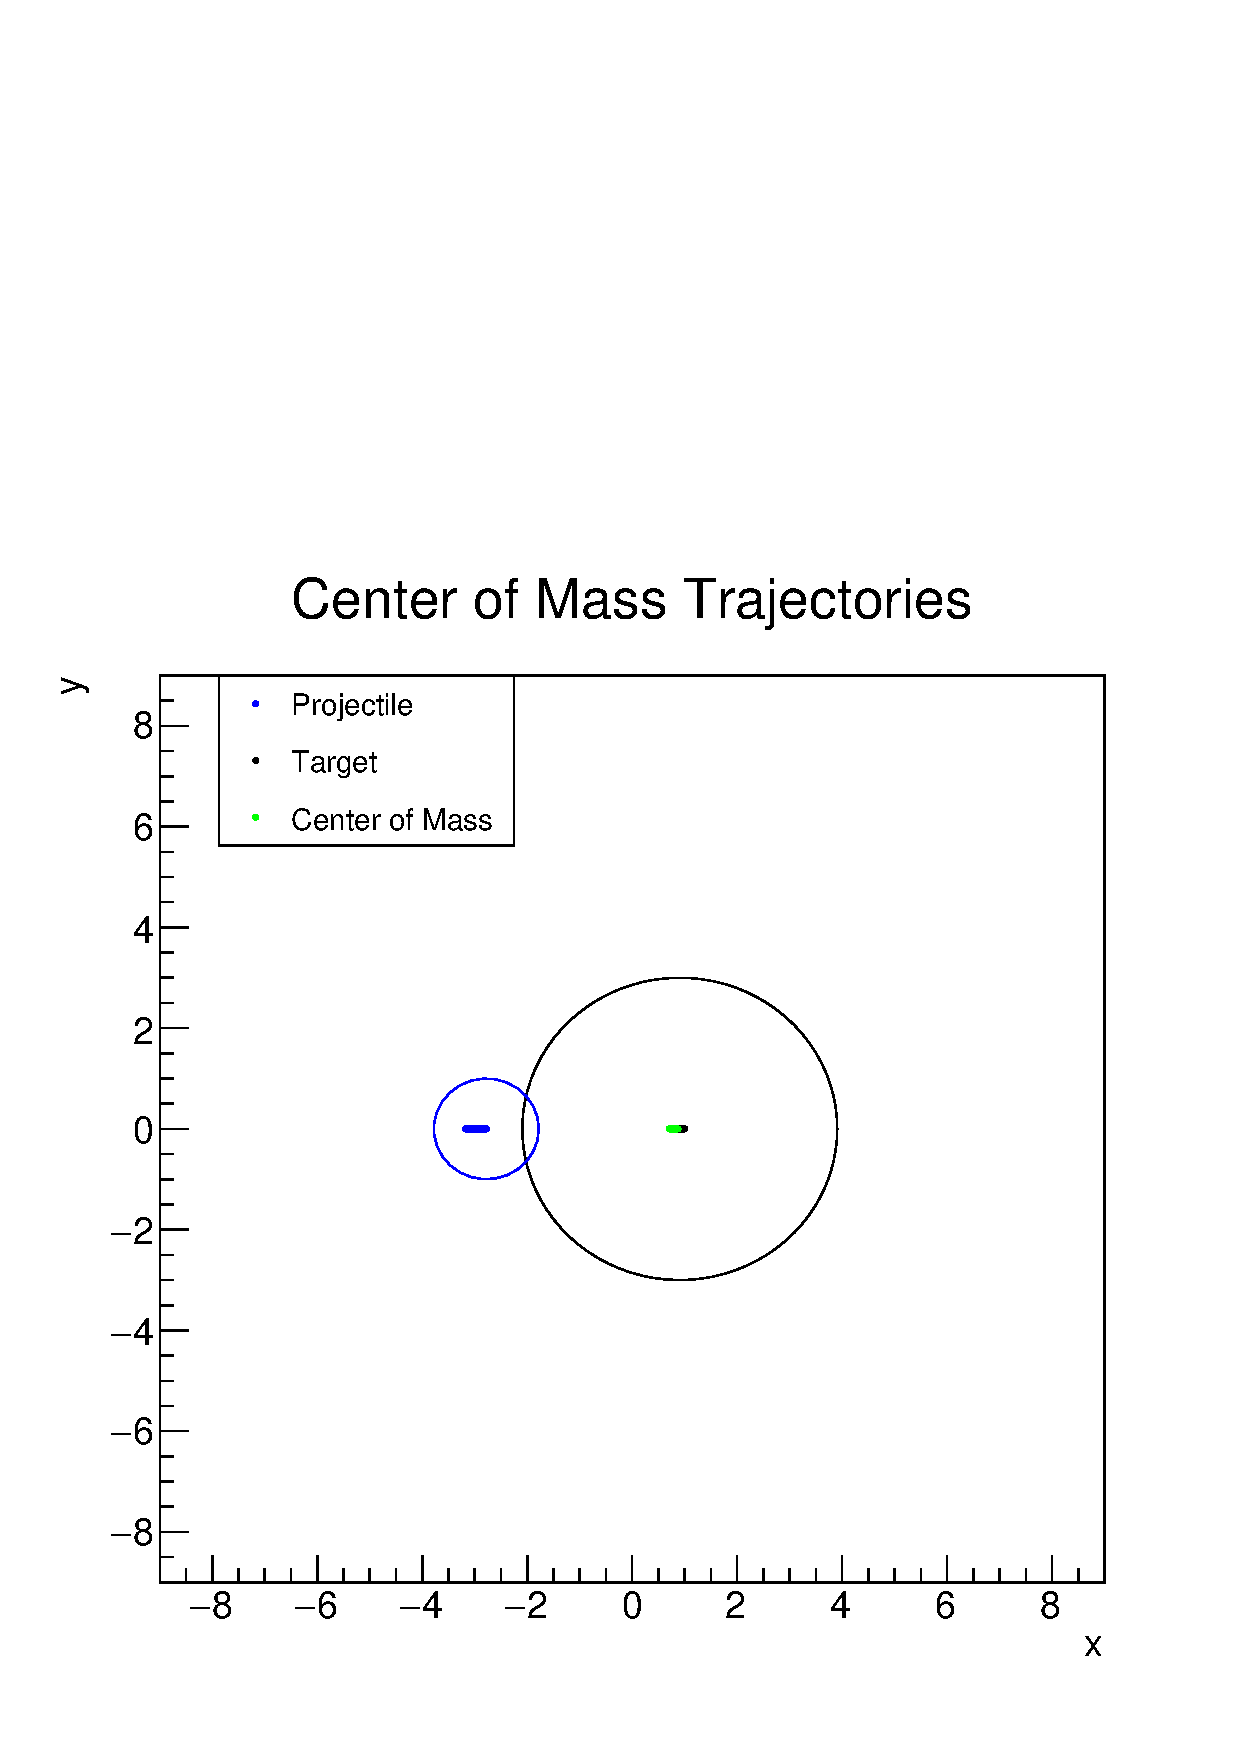
\includegraphics[width=.45\textwidth]{plots/out_c7/x_vs_y_with_ellipse_MS.pdf}
                  {\par\nobreak\rule[9pt]{35em}{0.5pt}\vspace{-5mm}}
                  \caption{(L) Object initial state, with tracks points (R) Objects at minimum separation, with track points}
                  \label{fig:tracks_c7}
\end{figure}
\begin{figure}[h!]
  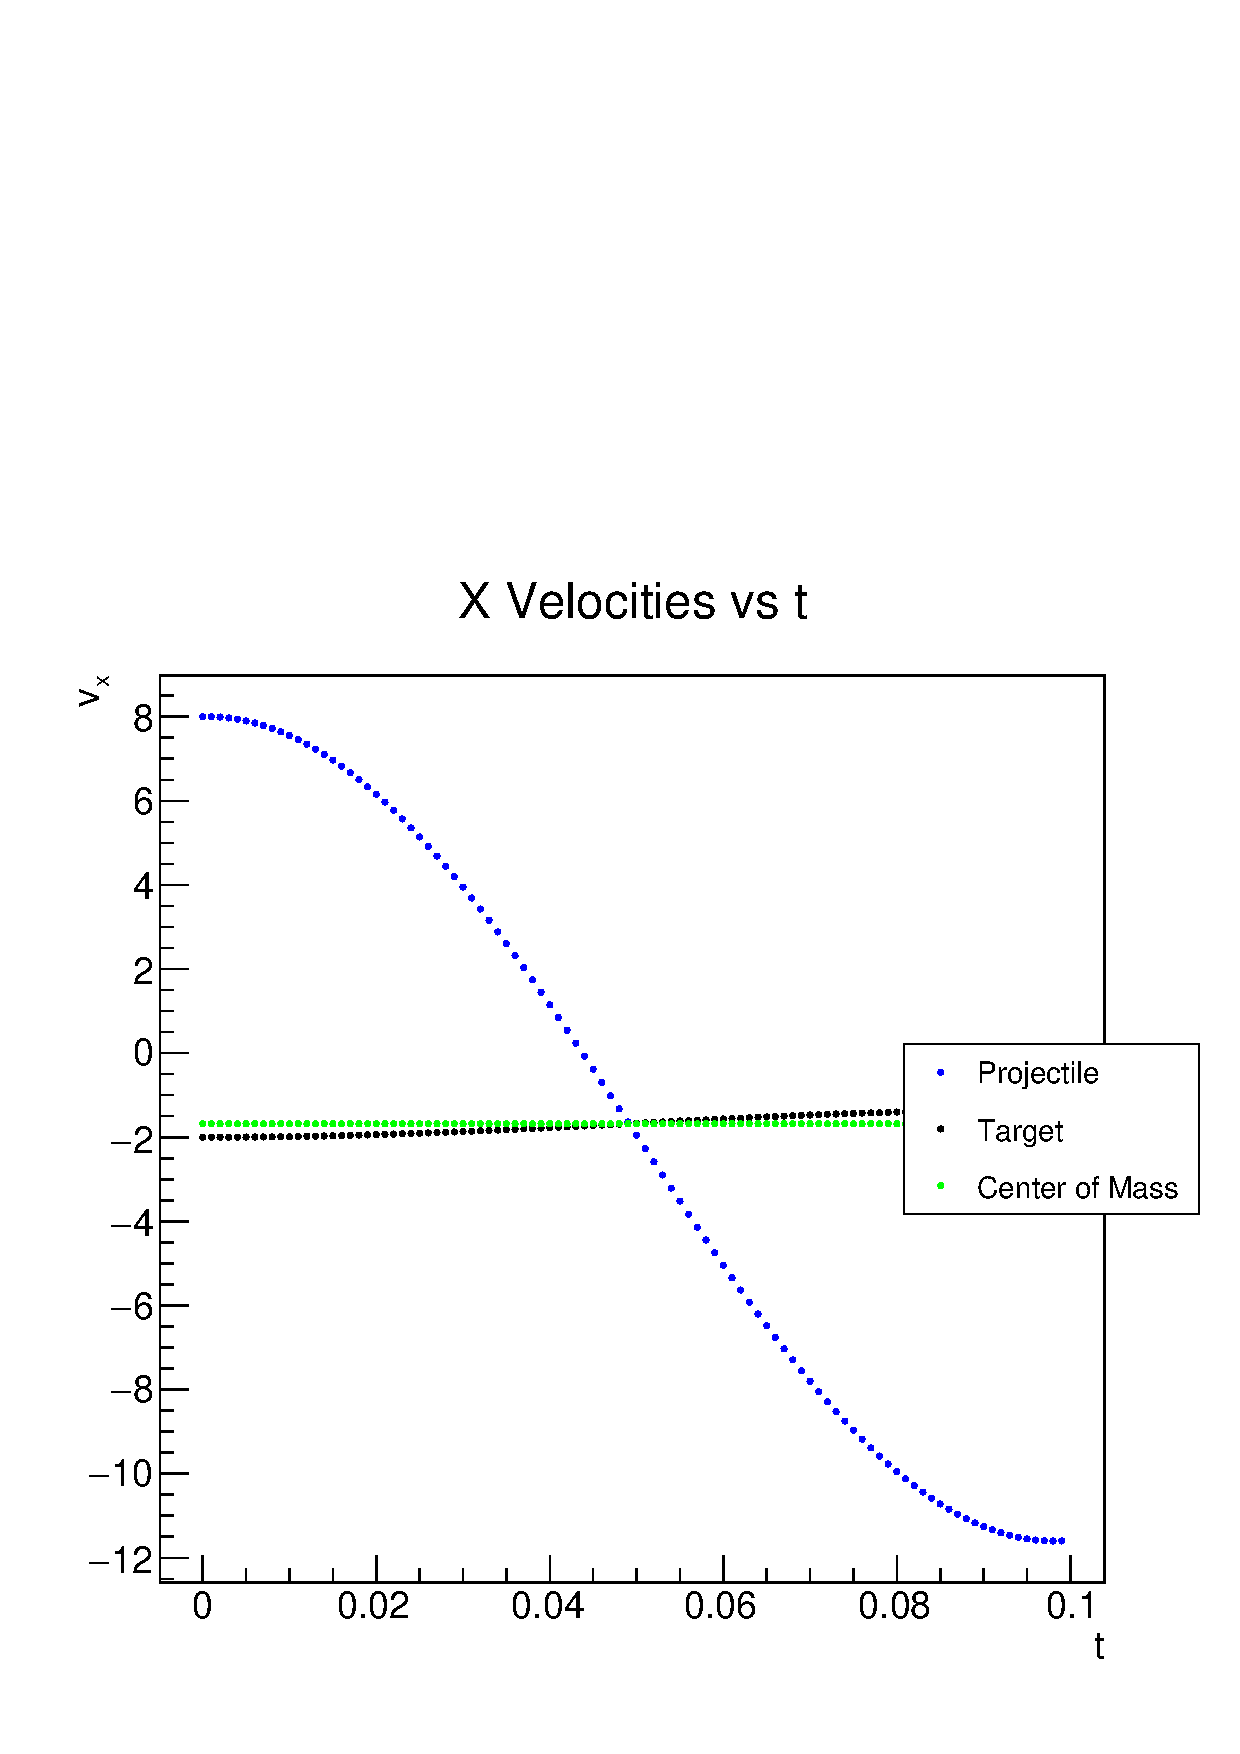
\includegraphics[width=.45\textwidth]{plots/out_c7/vx_vs_t.pdf}
                  {\par\nobreak\rule[9pt]{35em}{0.5pt}\vspace{-5mm}}
                  \caption{The velocity trend for each object and the center of mass. The velocity of the target is slightly changed, and stays in the same direction (to the left), while the incoming projectile is quickly turned around and given a larger velocity in the opposite direction compared to where it came out.}
                  \label{fig:vx_c7}
\end{figure}
%%%%%%%%%%%%%%%%%%%%%%%%%%%%%%%%%%%%%%%%%%%%%%%%%%%%%%%% trend studies %%%%%%%%%%%%%%%%%%%%%%%%%%%%%%%%%%%%%%%%%%%%%%%%%%%%%%%%%%%%%%%
\subsection{Initial Velocity Studies}
Many systems were simulated where we varied the initial velocity. Figure~\ref{fig:changing_pvinit1}(L) shows the maximum displacement from the ``spring'' equilibrium position versus initial velocity of the projectile. All of these systems were consistent in other parameters. This includes target radius and mass of 2, projectile radius of 0.25 and radius of 1 (equal densities). The impact parameter was 1, $\eta = 0$, and $\lambda = 1$. The asymptote at $\Delta x_{\text{max}}/r_t$ at 1 shows that as the initial velocity of the projectile increases, the impact reaches the radius of the target. Figure~\ref{fig:changing_pvinit1}(R) shows the energy loss per initial energy for the sample of systems. A perfect system would have a flat line at zero, but we are using finite time steps with this computational approximaton, therefore we have a slight gain in energy for low initial velocities. Figure~\ref{fig:energy_default} shows a a small increase in total energy for that particular system.
\begin{figure}[h!]
  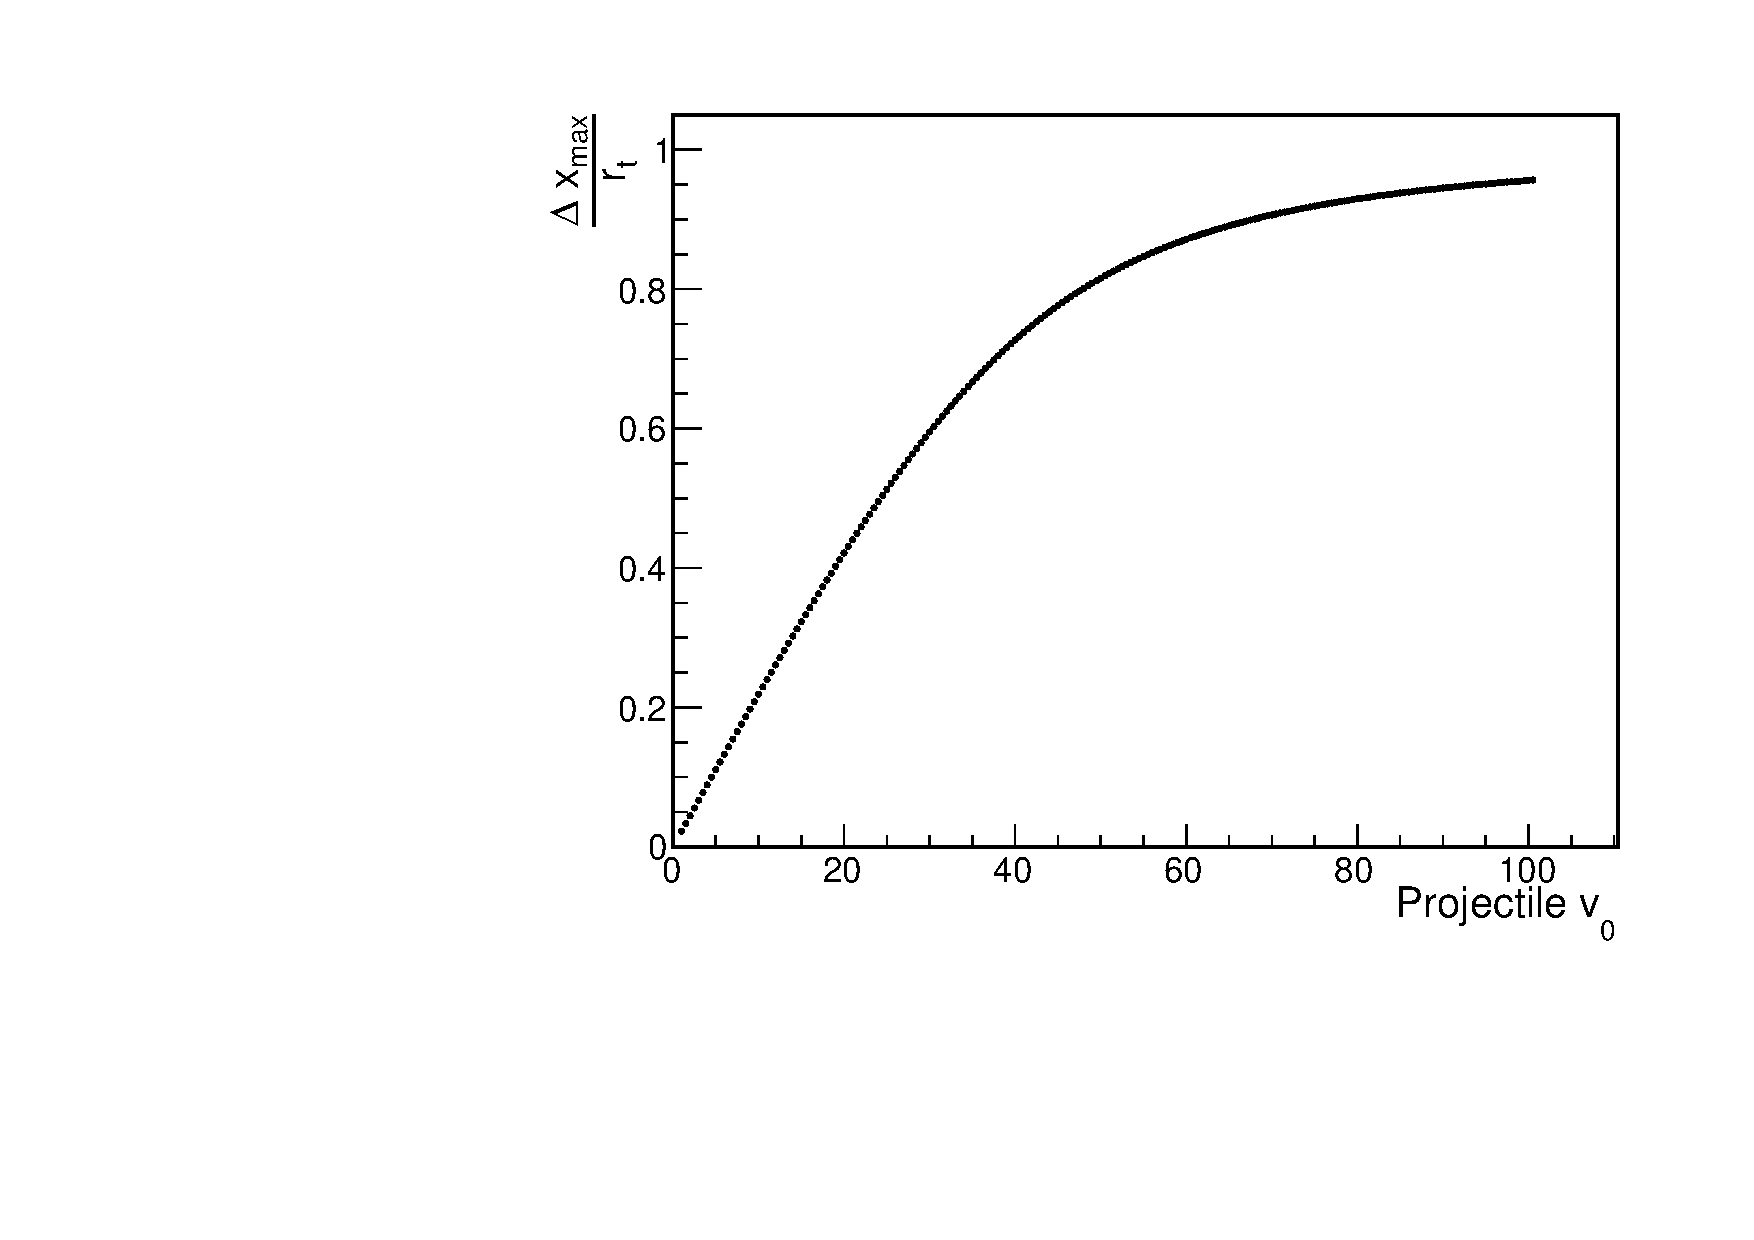
\includegraphics[width=.45\linewidth]{plots/trend_plots/dxmax_vs_pvinit.pdf}
  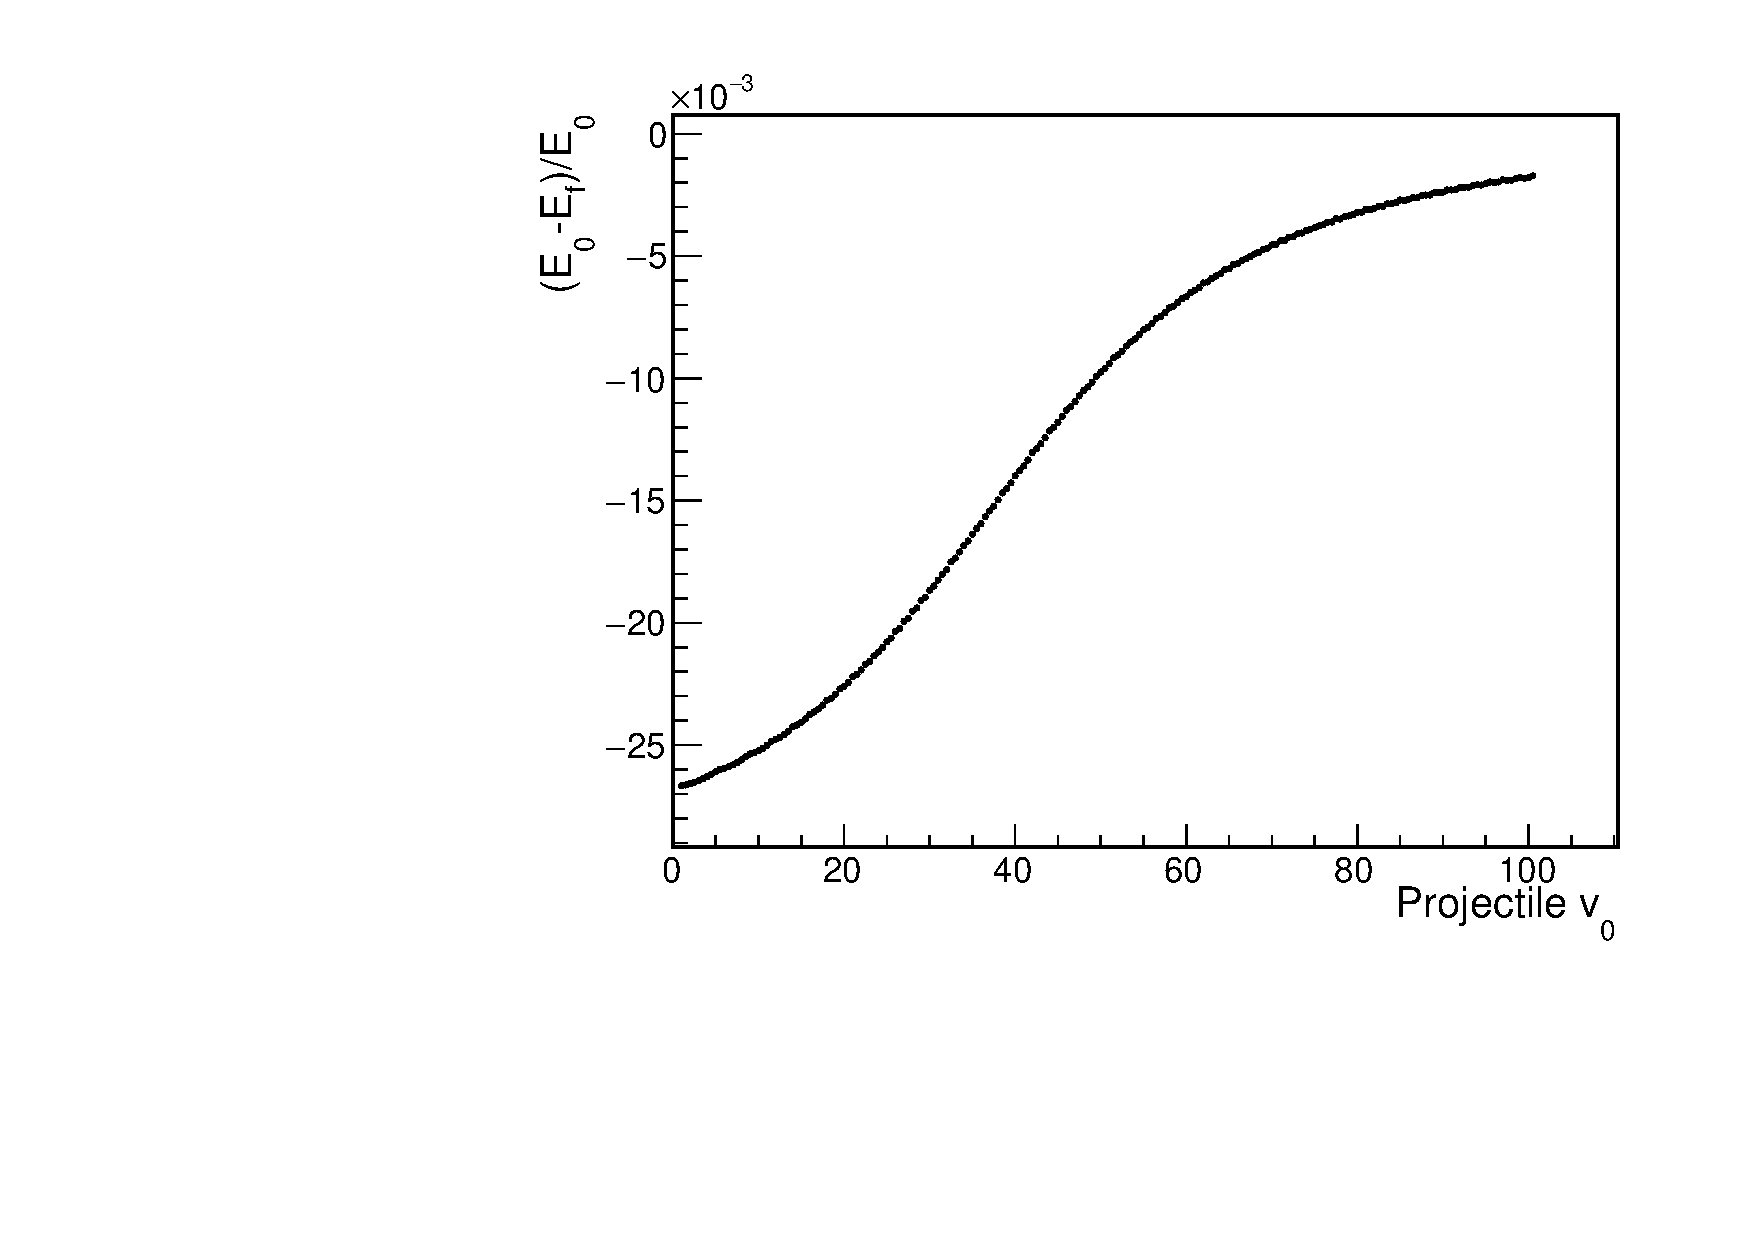
\includegraphics[width=.45\linewidth]{plots/trend_plots/Eloss_vs_pvinit.pdf}
                  {\par\nobreak\rule[9pt]{35em}{0.5pt}\vspace{-5mm}}
                  \caption{(L) The maximum displacement from equilibrium per target radius vs. the initial velocity of the projectile. (R) The energy loss divided by the initial energy of the system vs. initial velocity of the projectile.}
                  \label{fig:changing_pvinit1}
\end{figure}

\subsection{Impact Parameter Studies}
Many systems were simulated where we varied the impact parameter. Similar to the previous study, we again look at the trend of maximum displacement from equilibrium versus the varying parameter, which is now the impact parameter. During the generation of this sample, all other paramters were constant: target radius and mass of 2, projectile radius of 0.25 and radius of 1 (equal densities). The projectile initial velocity was 5, $\eta = 0$, and $\lambda = 1$. The trend shows that as the collision point becomes more off-center with respect to the target, the smaller the spring action between the two objects.
\begin{figure}[h!]
  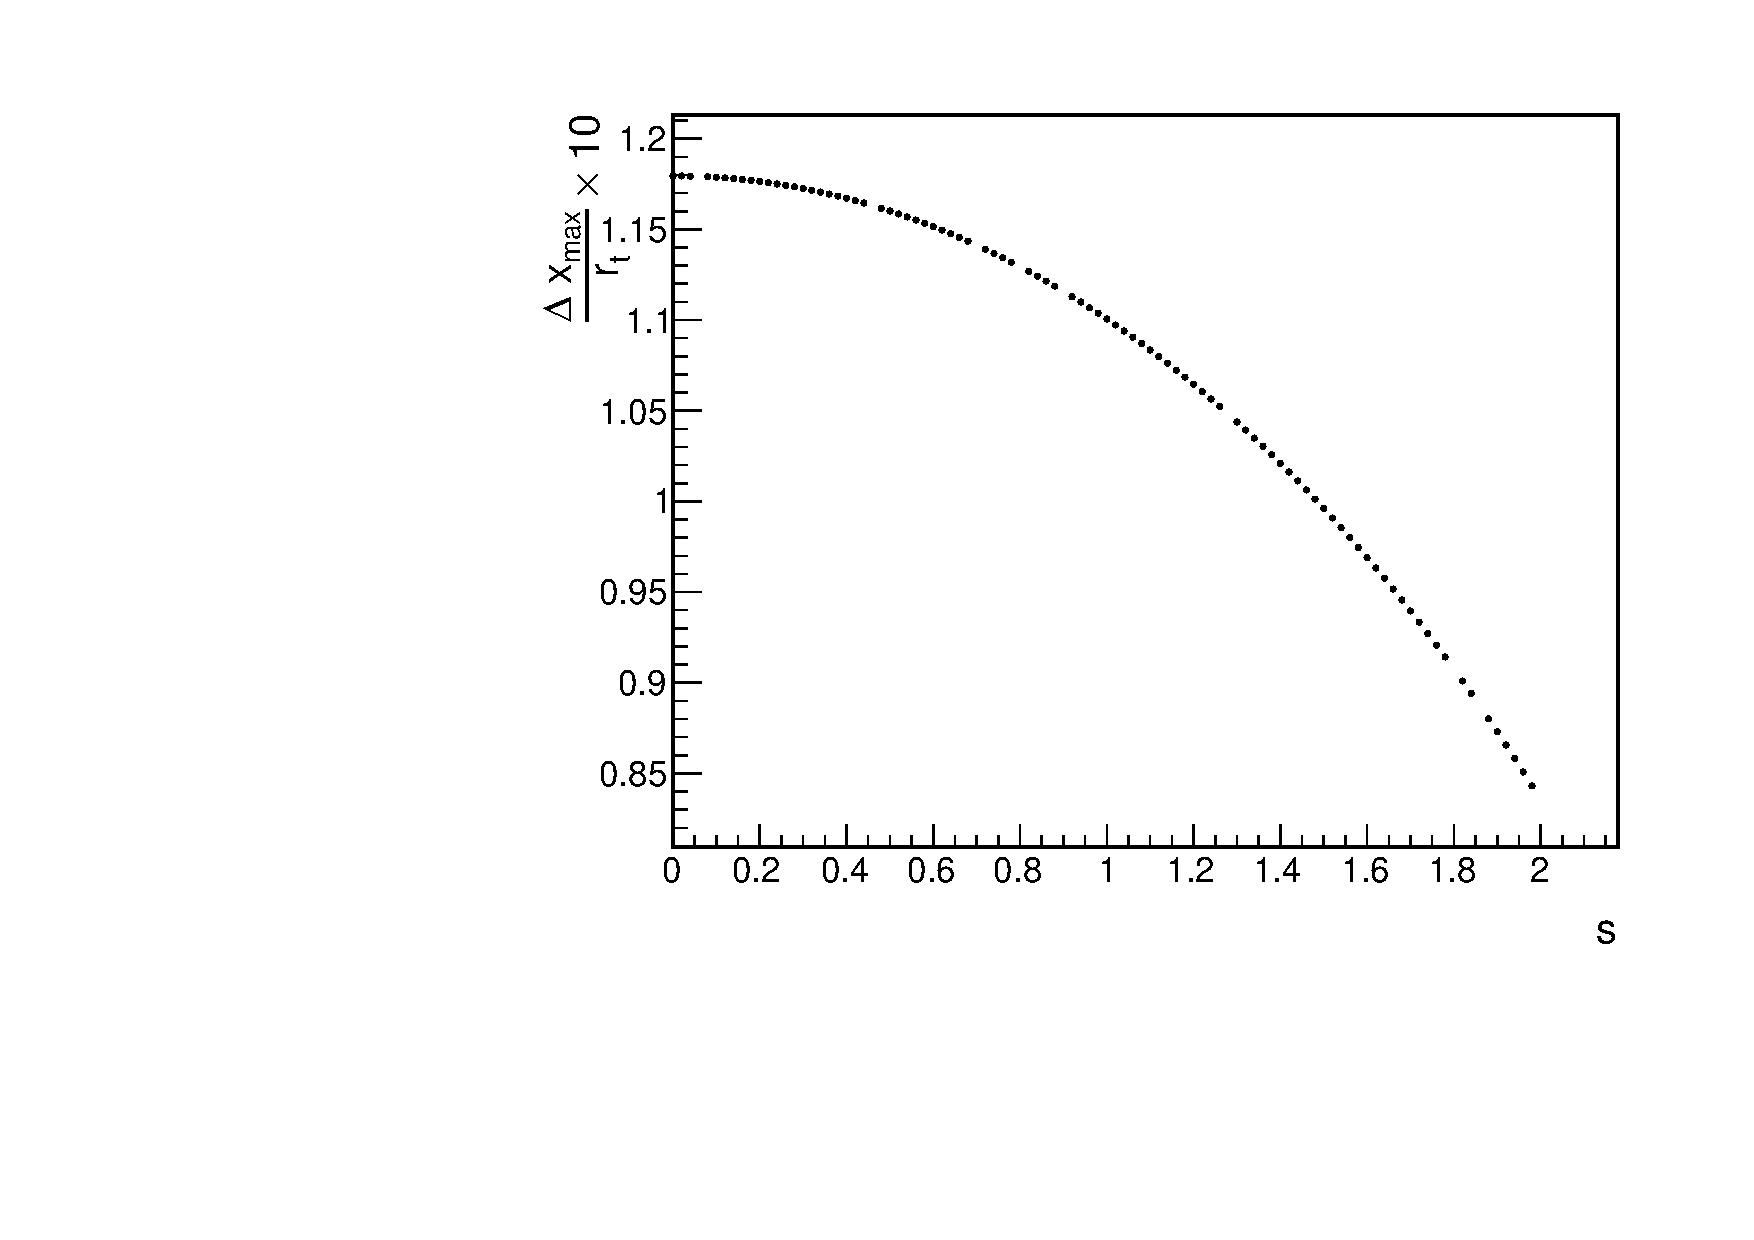
\includegraphics[width=.45\linewidth]{plots/trend_plots/Eloss_vs_s.pdf}
                  {\par\nobreak\rule[9pt]{35em}{0.5pt}\vspace{-5mm}}
                  \caption{The maximum displacement from equilibrium per the target radius vs. impact parameters.}
                  \label{fig:changing_s1}  
\end{figure}
Figure~\ref{fig:changing_s2} shows the trend of the final velocities of the objects versus the impact parameter. We find that for more head on collisions, the projectile transfers more momentum to the target, while for large impact parameters the projectile keeps most of its momentum.
\begin{figure}[h!]
  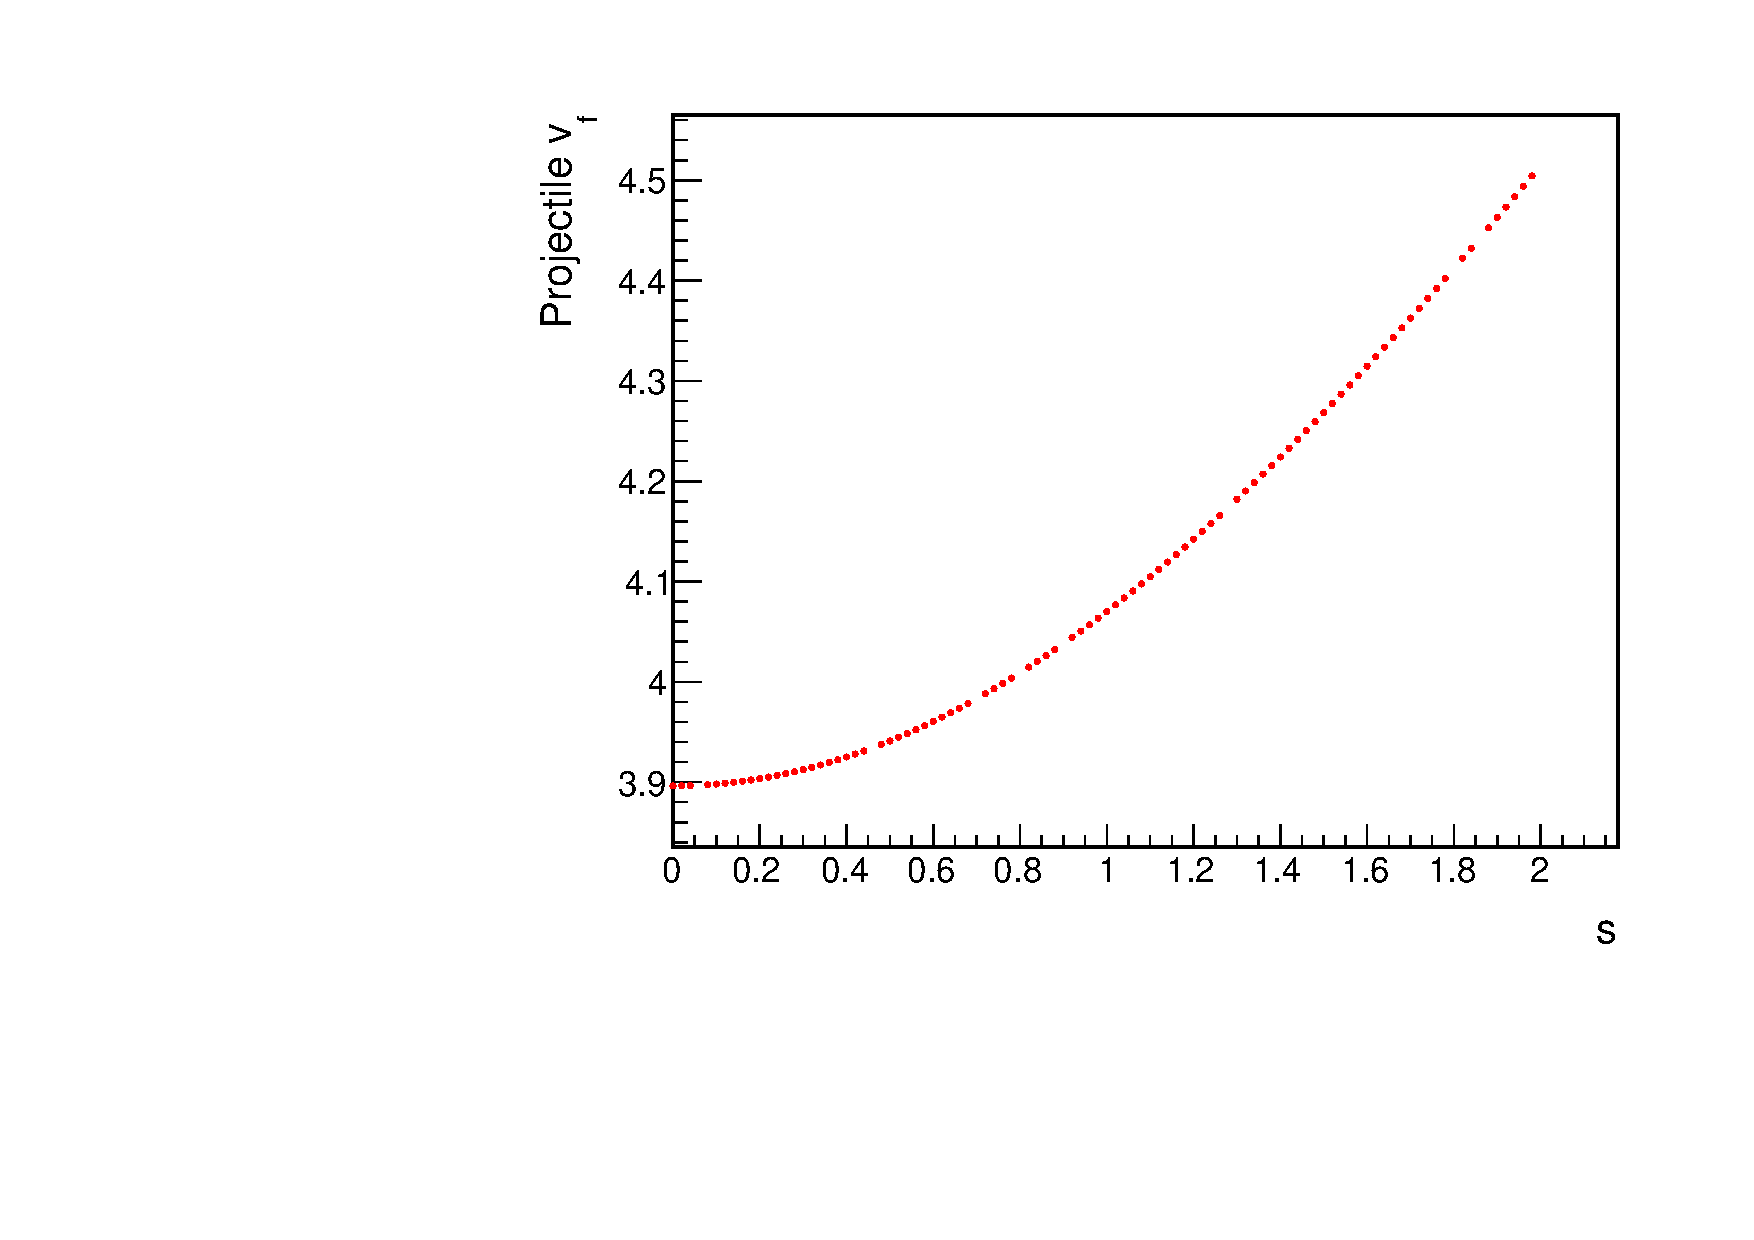
\includegraphics[width=.45\linewidth]{plots/trend_plots/pvf_vs_s.pdf}
  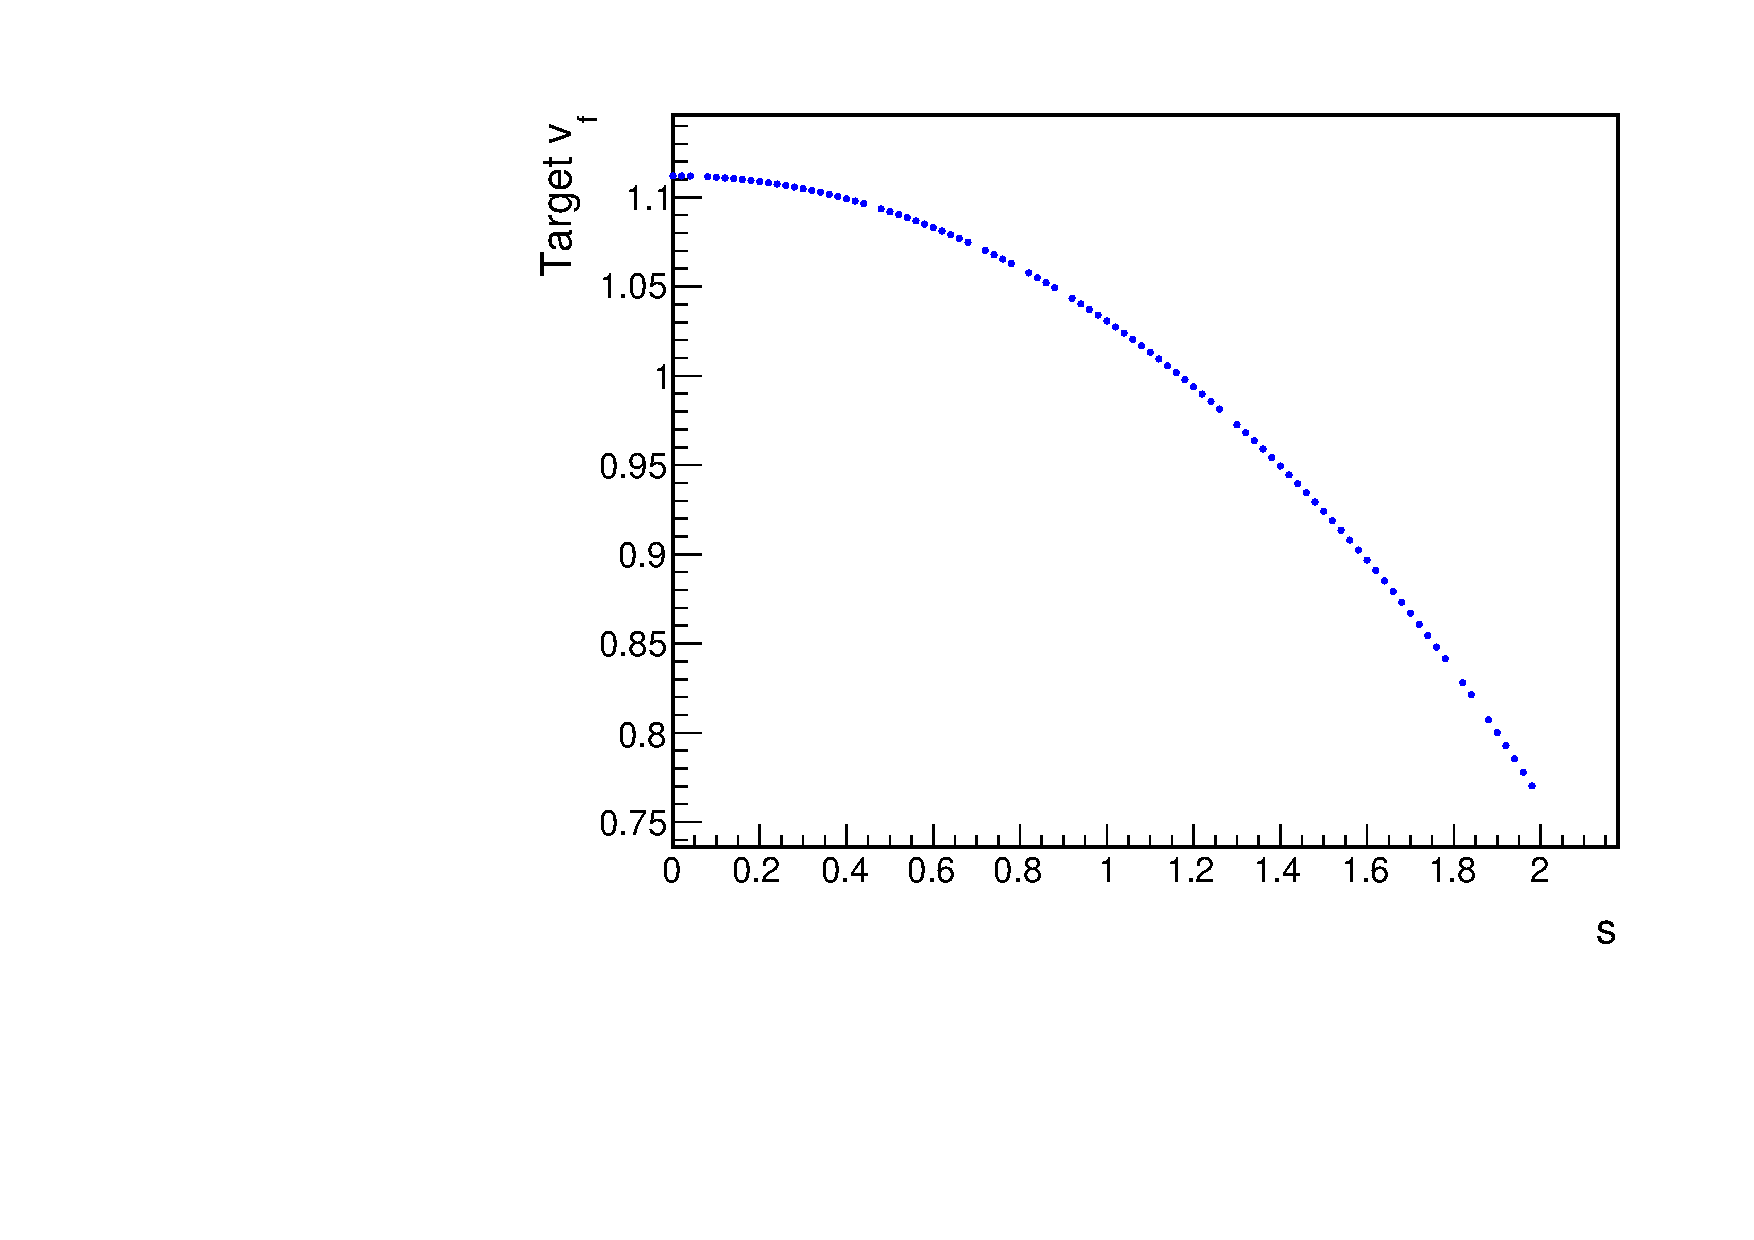
\includegraphics[width=.45\linewidth]{plots/trend_plots/tvf_vs_s.pdf}
                  {\par\nobreak\rule[9pt]{35em}{0.5pt}\vspace{-5mm}}
                  \caption{(L) The projectile final velocity vs. impact parameters. (R) The target final velocity vs. impact parameters.}
                  \label{fig:changing_s2}
\end{figure}

\subsection{Force Power Law Dependence}
Many systems were simulated where we varied the force power law parameter $\lambda$. We varied $\lambda$ from $1/2$ to $3$, which corresponds to a force law depending on the square root of the displacement up to depending on the cube of the displacement. Figure~\ref{fig:changing_lambda} shows this sample of maximum displacement from equilibrium versus the force law power. The trend has a positive slope throughout. This is unexpected, as we thought a larger $\lambda$ would correspond to a stronger restoring force between the objects, causing a smaller deformation. We now believe this is because all of the displacement values, $\Delta x$, are less than 1.
\begin{figure}[h!]
  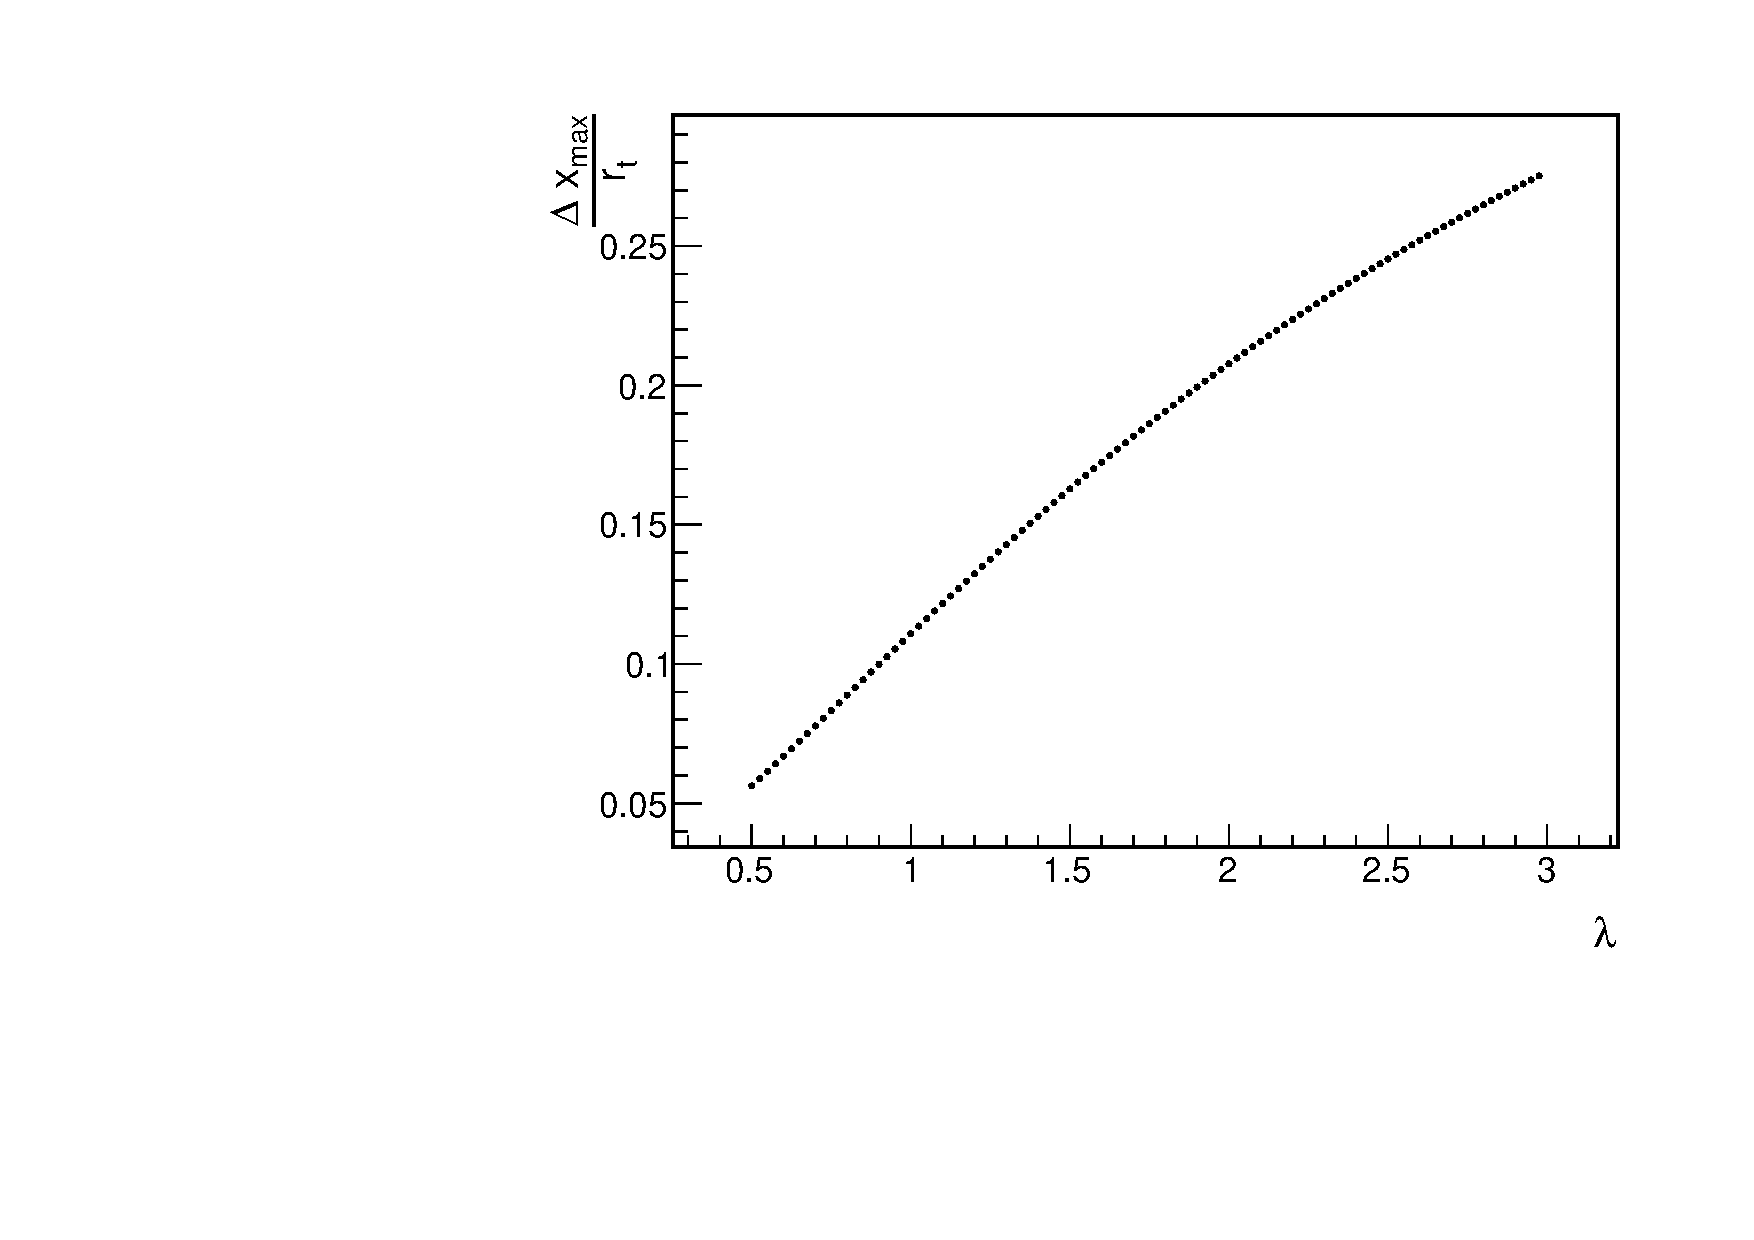
\includegraphics[width=.45\linewidth]{plots/trend_plots/dxmax_vs_lambda.pdf}
                  {\par\nobreak\rule[9pt]{35em}{0.5pt}\vspace{-5mm}}
                  \caption{The maximum displacement from equilibrium per target radius vs. $\lambda$}
                  \label{fig:changing_lambda}
\end{figure}

\subsection{Energy Dissipation Studies}
Many systems were simulated where we varied the energy dissipation parameter $\eta$. Figure~\ref{fig:changing_eta}.
\begin{figure}[h!]
  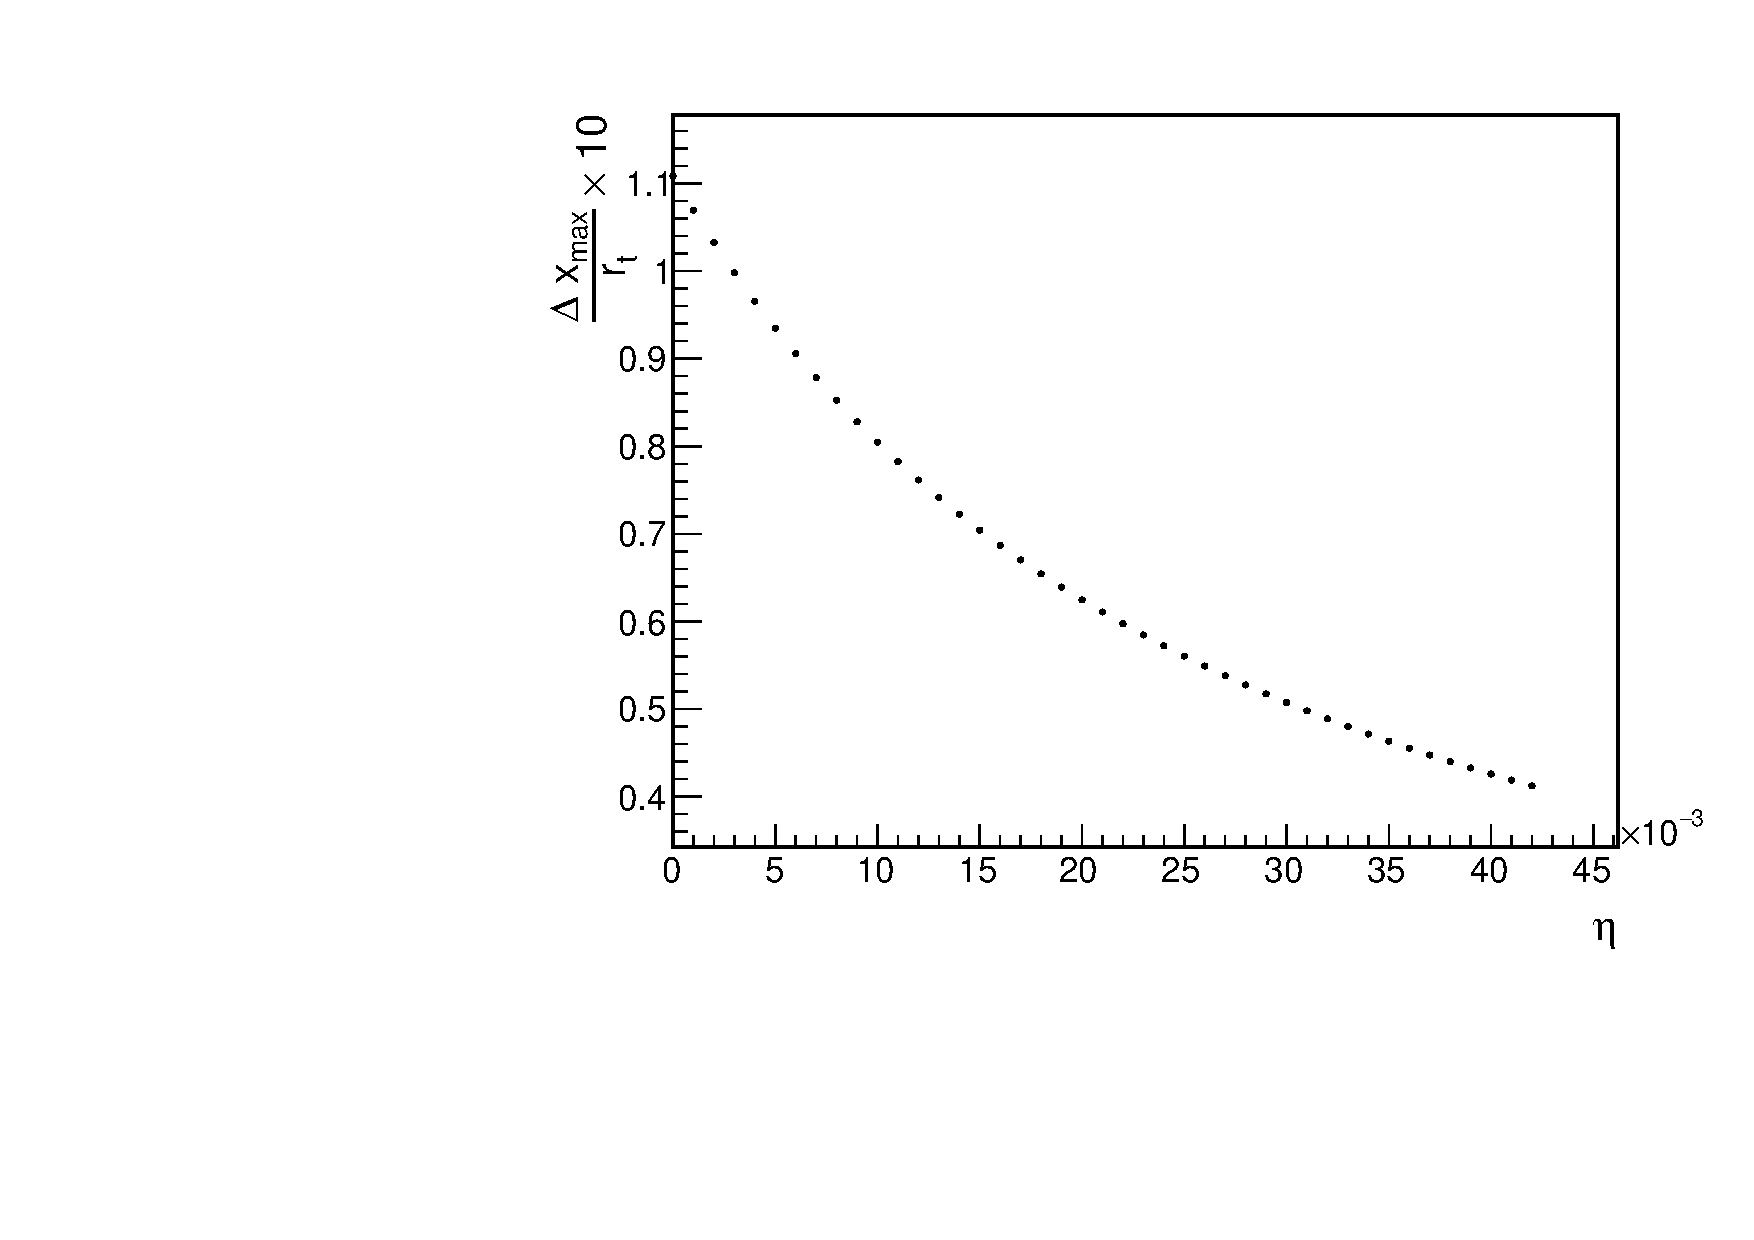
\includegraphics[width=.45\linewidth]{plots/trend_plots/dxmax_vs_eta.pdf}
  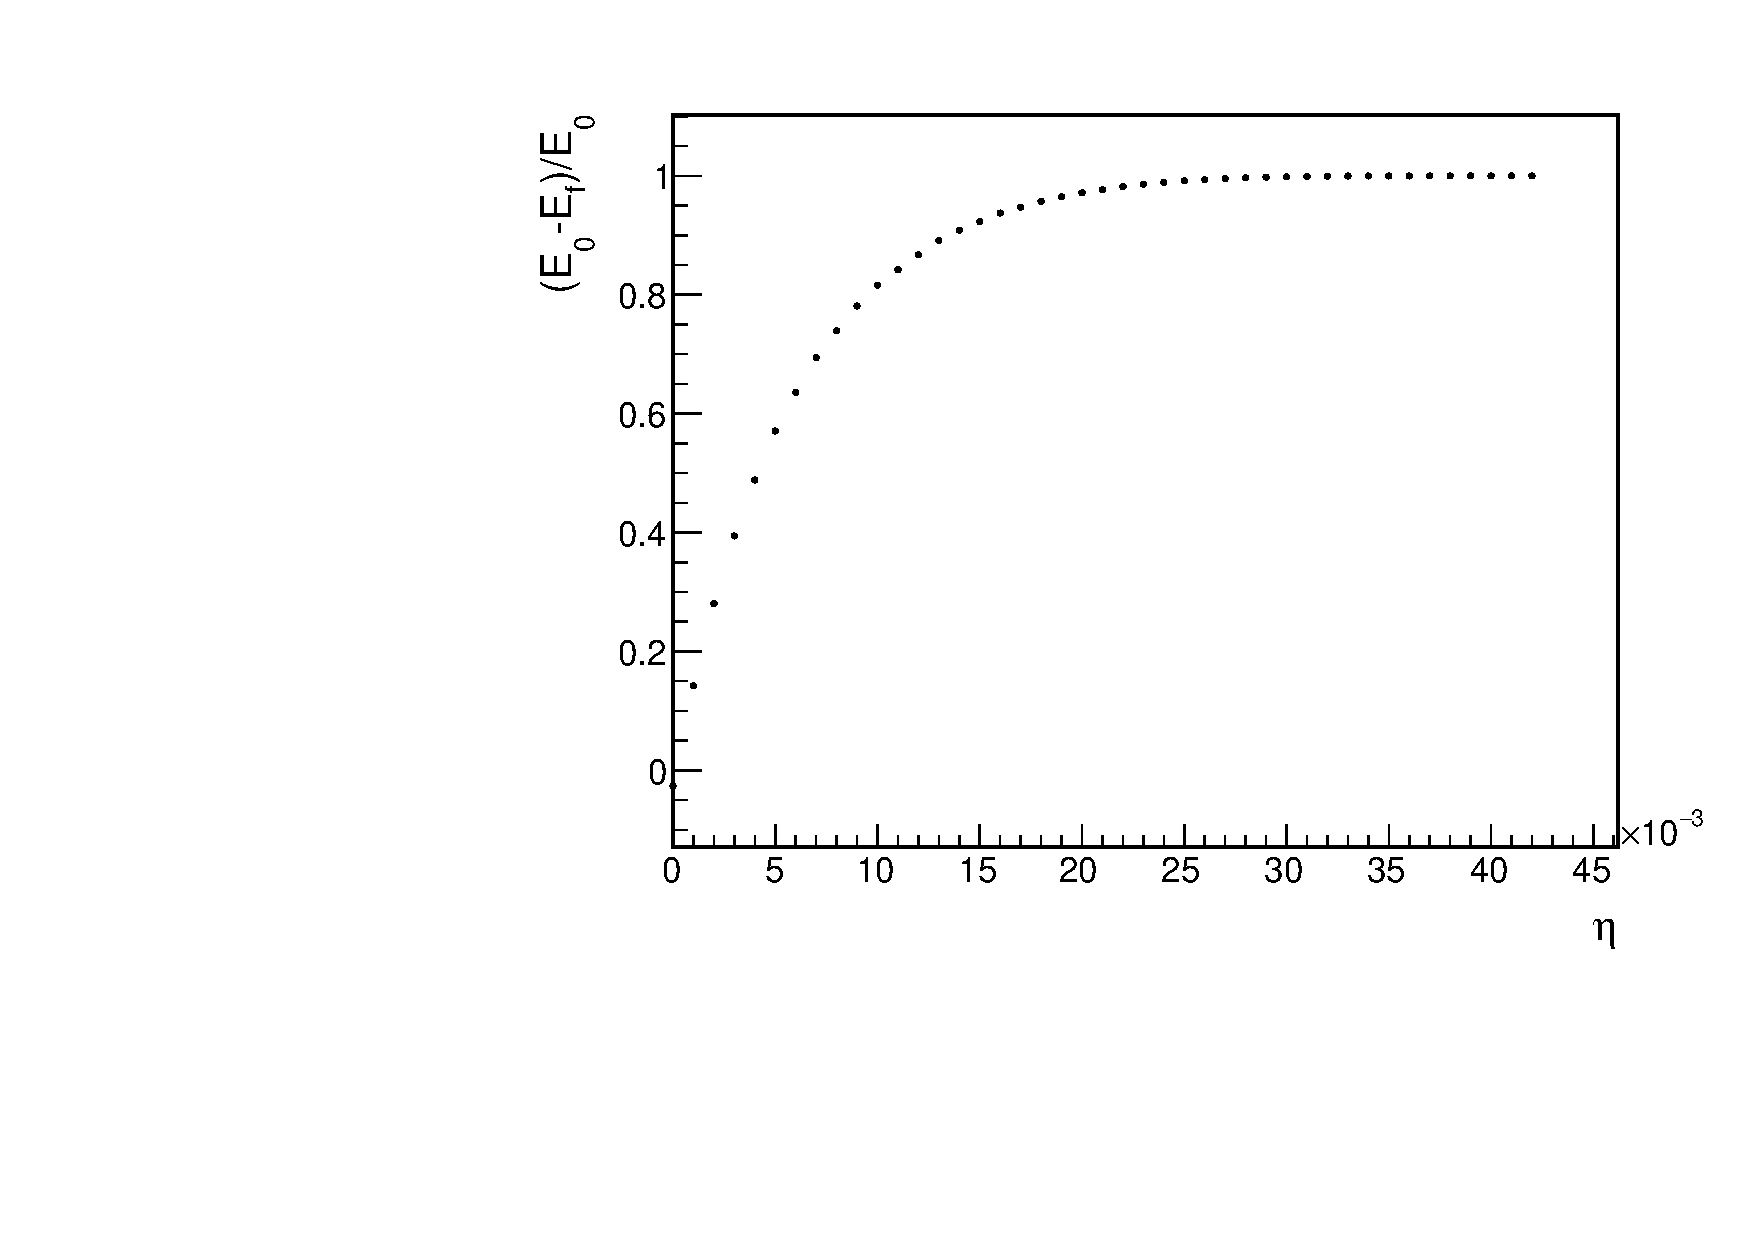
\includegraphics[width=.45\linewidth]{plots/trend_plots/Eloss_vs_eta.pdf}
                  {\par\nobreak\rule[9pt]{35em}{0.5pt}\vspace{-5mm}}
                  \caption{(L) the maximum displacement from equilibrium per target radius vs. $\eta$. (R) The energy loss per initial energy vs. $\eta$.}
                  \label{fig:changing_eta}
\end{figure}


\section{Conclusion}
The

\clearpage
\begin{thebibliography}{9}
  \section{Bibliography}
\bibitem{ref_root}
  R.~Brun and F.~Rademakers, \emph{ROOT - An Object Oriented Data Analysis Framework}, Proceedings AIHENP 96 Workshop, Lausanne, Sep. 1996, Nucl. Inst. \& Meth. in Phys. Res. A 389 (1997) 81-86. See also http://root.cern.ch/.

\end{thebibliography}

\clearpage
%\begin{appendices}
%  \singlespacing
%  \section{main.cpp Physics Loop} \label{sec:main.cpp}
%  \lstinputlisting[firstline=170, lastline=246]{../main.cpp}% lots of pages, only uncomment when you want it

%\end{appendices}

\end{document}
